\chapter{Analyse et spécification des besoins}

\section*{Introduction}
L'analyse des besoins transforme le périmètre présenté au chapitre précédent en attentes vérifiables, cas d'utilisation et règles de gestion. Elle s'appuie ici sur le comportement du dépôt JobTest : interface Next.js, routes FastAPI effectivement sollicitées, persistance et moteur de décision. L'objectif n'est pas de décrire une plateforme RH générique, mais de fixer le contrat fonctionnel de l'application démontrable. Après la délimitation du système et l'identification de ses parties prenantes, le chapitre spécifie les besoins, les contraintes de qualité, les règles de gestion, les cas d'utilisation et leur traçabilité.

\section{Périmètre fonctionnel de JobTest}
JobTest est une application d'aide à la présélection destinée au recruteur. Elle organise des offres et des dossiers candidats, puis fournit une évaluation hybride entre un CV et une offre. Le résultat associe une recommandation officielle, ses composantes, les compétences détectées ou manquantes et des éléments d'explication. L'analyse qualitative produite par le LLM local complète cette restitution sans participer à la décision officielle.

Le périmètre couvert comprend l'inscription et la session du recruteur, la gestion des offres et des candidats, l'évaluation d'un texte ou d'un document PDF/DOCX, la consultation des résultats et de l'historique, le classement multi-CV, l'export PDF, la comparaison ponctuelle des méthodes, le centre de qualité hors ligne et le réglage de seuils pour la session. Les données opérationnelles et les résultats persistés sont isolés par recruteur.

Sont hors périmètre une décision d'embauche autonome, un portail candidat, la conduite des entretiens et un apprentissage sur des résultats réels d'embauche. JobTest ne remplace donc pas l'appréciation du recruteur ni les étapes humaines de sélection. Son benchmark repose sur des données synthétiques. Enfin, le déploiement Azure validé est une démonstration PFE sur une instance sans haute disponibilité permanente ; il ne constitue pas une offre de production 24/7.

\section{Identification des acteurs et parties prenantes}
\subsection{Visiteur non authentifié}
Avant l'authentification, le visiteur peut créer un compte recruteur ou se connecter. Aucun parcours public de consultation d'offres, de dépôt de candidature, de réinitialisation de mot de passe, de vérification d'e-mail ou de connexion sociale n'a été retenu, car il n'est pas exposé par l'application actuelle.

\subsection{Recruteur authentifié}
Le recruteur est l'acteur opérationnel principal. Une fois la session JWT établie, il consulte le tableau de bord et gère ses propres offres, candidats et résultats. Il peut évaluer un CV, consulter le résultat explicable, demander l'analyse approfondie facultative, exporter un rapport, classer plusieurs CV, consulter l'historique, comparer les méthodes, visualiser la qualité hors ligne et modifier les seuils actifs de sa session. Les contrôles d'appartenance empêchent l'accès aux objets d'un autre recruteur.

\subsection{Candidat en tant qu'entité métier}
Le candidat est le sujet d'une évaluation et une entité persistée : identité facultative, coordonnées, statut de pipeline, CV et résultats associés. Il n'est pas un acteur logiciel interactif. La version étudiée ne fournit ni compte candidat ni écran candidat ni soumission publique de CV. Cette séparation évite de confondre l'objet métier évalué avec l'utilisateur autorisé à utiliser l'application.

\subsection{Partie prenante technique}
Une personne chargée de maintenance ou d'assurance qualité peut exécuter le benchmark hors ligne, exporter ses figures ou intervenir sur l'environnement. Cette partie prenante est technique et secondaire : aucun portail administrateur, rôle d'administration distinct ni parcours d'authentification administrateur n'est prouvé dans l'interface opérationnelle. Elle ne figure donc pas comme acteur du diagramme global.

Le tableau~\ref{tab:acteurs-jobtest} récapitule ces acteurs et situe chacun d'eux par rapport au parcours métier.

\begin{table}[htbp]
\centering\small
\begin{tabularx}{\textwidth}{|p{3.2cm}|p{2.5cm}|X|p{3.1cm}|}
\hline
\textbf{Élément} & \textbf{Type} & \textbf{Rôle} & \textbf{Accès au système}\\
\hline
Visiteur non authentifié & Acteur & Crée un compte ou amorce une session & Écran d'accès, sans données métier\\
\hline
Recruteur authentifié & Acteur & Gère et évalue ses dossiers & Toutes les fonctions métier après JWT\\
\hline
Candidat & Entité métier & Porte le CV, le pipeline et les résultats & Aucun accès interactif\\
\hline
Maintenance / QA & Partie prenante technique & Produit ou contrôle le benchmark hors ligne & Hors parcours métier courant\\
\hline
\end{tabularx}
\caption{Acteurs et parties prenantes de JobTest}
\label{tab:acteurs-jobtest}
\end{table}

\section{Spécification des besoins fonctionnels}
Les besoins sont présentés par domaine afin de décrire le parcours réellement disponible, sans confondre les fonctions du recruteur avec une décision autonome de recrutement.


Le tableau~\ref{tab:besoins-fonctionnels} énumère ces besoins avec leur identifiant, l'acteur concerné et le critère qui permet d'en constater la réalisation.

{\footnotesize\setlength{\tabcolsep}{2pt}
\begin{longtable}{|>{\raggedright\arraybackslash\scriptsize}p{2.15cm}|>{\raggedright\arraybackslash}p{4.05cm}|>{\raggedright\arraybackslash}p{1.9cm}|>{\raggedright\arraybackslash}p{1.8cm}|>{\raggedright\arraybackslash}p{3.55cm}|}
\caption{Besoins fonctionnels de JobTest}\label{tab:besoins-fonctionnels}\\
\hline
\textbf{Identifiant} & \textbf{Besoin fonctionnel} & \textbf{Acteur} & \textbf{Priorité} & \textbf{Critère d'acceptation}\\
\hline
\endfirsthead
\hline
\textbf{Identifiant} & \textbf{Besoin fonctionnel} & \textbf{Acteur} & \textbf{Priorité} & \textbf{Critère d'acceptation}\\
\hline
\endhead
BF-AUTH-01 & Créer un compte recruteur avec nom, e-mail et mot de passe. & Visiteur & Essentiel & Un compte de rôle \texttt{recruiter} est créé ; un e-mail déjà utilisé est refusé.\\
\hline
BF-AUTH-02 & S'authentifier et récupérer l'utilisateur courant. & Visiteur & Essentiel & Les identifiants valides donnent un JWT bearer puis le profil \texttt{/auth/me}.\\
\hline
BF-AUTH-03 & Clore la session côté interface. & Recruteur & Essentiel & Le jeton local est supprimé lors de la déconnexion.\\
\hline
BF-JOB-01 & Créer et lister ses offres. & Recruteur & Essentiel & Titre et description sont exigés ; un code \texttt{JOB-YYYY-NNN} est attribué.\\
\hline
BF-JOB-02 & Modifier une offre possédée et son statut. & Recruteur & Essentiel & Les statuts admis sont \texttt{OPEN}, \texttt{ON\_HOLD} et \texttt{CLOSED}.\\
\hline
BF-JOB-03 & Basculer rapidement l'ouverture d'une offre. & Recruteur & Compl. & L'action dédiée alterne \texttt{OPEN} et \texttt{CLOSED}.\\
\hline
BF-JOB-04 & Supprimer une offre non évaluée. & Recruteur & Essentiel & La suppression est refusée si des évaluations sont liées ; l'offre peut alors être clôturée.\\
\hline
BF-CAND-01 & Consulter ses candidats. & Recruteur & Essentiel & La liste est filtrée par propriétaire et expose activité, meilleur score et statut.\\
\hline
BF-CAND-02 & Mettre à jour identité, contact et pipeline. & Recruteur & Essentiel & Nom obligatoire ; statuts admis : \texttt{NEW}, \texttt{UNDER\_REVIEW}, \texttt{SHORTLISTED}, \texttt{INTERVIEW}, \texttt{HIRED}, \texttt{REJECTED}.\\
\hline
BF-CAND-03 & Supprimer un candidat sans résultat lié. & Recruteur & Essentiel & Une suppression avec évaluation est refusée ; le recruteur peut modifier le statut du pipeline.\\
\hline
BF-EVAL-01 & Évaluer du texte CV contre une offre possédée. & Recruteur & Essentiel & Le CV contient au moins cinq mots ; méthode, score, décision et explication sont retournés et persistés.\\
\hline
BF-EVAL-02 & Évaluer un PDF ou DOCX. & Recruteur & Essentiel & Seuls PDF et DOCX sont acceptés ; un texte lisible est extrait avant l'évaluation.\\
\hline
BF-EVAL-03 & Afficher le résultat explicable. & Recruteur & Essentiel & Verdict \texttt{HIRE}/\texttt{CONSIDER}/\texttt{REJECT}, composantes, compétences, écarts, recommandations et données radar sont restitués.\\
\hline
BF-LLM-01 & Demander séparément une analyse approfondie. & Recruteur & Compl. & La requête cible un \texttt{MatchResult} possédé ; son état peut être \texttt{ok}, désactivé, indisponible ou en erreur.\\
\hline
BF-REPORT-01 & Générer et télécharger un rapport PDF depuis un résultat. & Recruteur & Compl. & Le navigateur reçoit un document PDF à partir du résultat et de son explication.\\
\hline
BF-RANK-01 & Classer plusieurs CV pour une offre. & Recruteur & Compl. & Des fichiers PDF/DOCX sont évalués pour une offre sélectionnée, puis ordonnés par score décroissant.\\
\hline
BF-RANK-02 & Exporter le classement courant. & Recruteur & Compl. & L'interface produit un CSV côté navigateur ; il ne crée pas un nouvel enregistrement métier.\\
\hline
BF-HIST-01 & Consulter l'historique et le détail d'une évaluation. & Recruteur & Essentiel & Les résultats propres au recruteur sont listés, filtrables et consultables par identifiant.\\
\hline
BF-QUALITY-01 & Comparer les méthodes en direct. & Recruteur & Compl. & \textit{AI Insights} compare les méthodes sur un CV/offre fourni sans persister de \texttt{MatchResult}.\\
\hline
BF-QUALITY-02 & Consulter le benchmark hors ligne. & Recruteur & Compl. & \textit{AI Quality Center} affiche des données et figures file-backed avec leur disponibilité.\\
\hline
BF-SETTINGS-01 & Configurer les seuils de décision de la session. & Recruteur & Compl. & Les seuils Strong Fit et Potential Fit sont validés, transmis aux évaluations ultérieures et conservés dans celles-ci.\\
\hline
\end{longtable}\par}
\normalsize

\subsection{Authentification du recruteur}
\begin{itemize}
  \item Créer un compte recruteur avec nom, e-mail et mot de passe, en refusant un e-mail déjà utilisé.
  \item Se connecter, consulter son profil courant et fermer la session côté interface.
\end{itemize}

L'inscription crée uniquement un recruteur. La connexion utilise le formulaire OAuth2 de l'API, qui retourne un jeton bearer. L'interface conserve ce jeton pour appeler \texttt{/auth/me} et les routes protégées ; la déconnexion l'efface côté client. Aucun besoin de réinitialisation de mot de passe ou d'activation n'est spécifié car ces parcours ne sont pas présents.

\subsection{Gestion des offres et des candidats}
\begin{itemize}
  \item Créer, consulter, modifier, clôturer ou rouvrir ses propres offres ; le code est attribué automatiquement.
  \item Supprimer une offre seulement lorsqu'aucune évaluation ne lui est liée ; une offre évaluée peut être clôturée.
  \item Consulter les candidats du recruteur, mettre à jour leurs informations et leur statut de pipeline, puis supprimer un dossier sans résultat associé.
\end{itemize}

Les offres sont créées avec un titre, une description, des compétences requises facultatives et un statut. Le code est calculé automatiquement. Toutes les opérations vérifient le recruteur propriétaire. Une offre liée à des évaluations ne peut pas être supprimée, afin de préserver la cohérence de l'historique. L'évaluation crée ou réutilise le dossier candidat lorsque les informations disponibles le permettent ; la page candidats sert ensuite à la consultation et à la mise à jour. Les fonctions exposées dans l'interface courante sont la modification et la suppression conditionnelle. L'API historique comporte une anonymisation, mais elle n'est pas présentée comme un parcours du frontend Next.js faute d'action correspondante vérifiée.

\subsection{Évaluation et restitution}
\begin{itemize}
  \item Évaluer un texte CV ou un document PDF/DOCX par rapport à une offre possédée.
  \item Consulter le verdict, le score, les composantes, les compétences, les écarts et les recommandations enregistrés.
  \item Demander séparément une analyse approfondie locale ; son indisponibilité ne modifie pas le verdict officiel.
  \item Générer et télécharger le rapport PDF d'une évaluation.
\end{itemize}

Le recruteur sélectionne une offre qu'il possède, saisit éventuellement identité et e-mail, puis transmet du texte ou un fichier. La couche statistique lance l'appariement choisi, le \textit{DecisionEngine} applique les seuils actifs et le service persiste un résultat. Le résultat visible comprend le score global, les sous-scores, la décision, l'explication, les compétences et les écarts. L'analyse approfondie est une seconde demande sur une évaluation déjà persistée. Si Ollama est désactivé, indisponible ou en erreur, l'état est retourné sans bloquer ni altérer le verdict statistique. Seule une enveloppe avec état \texttt{ok} est sauvegardée. Le rapport PDF, enfin, réutilise les données déjà calculées et n'ouvre pas un nouveau calcul de correspondance.

\subsection{Historique, classement et réglages}
\begin{itemize}
  \item Consulter l'historique et le détail des évaluations appartenant au recruteur.
  \item Classer plusieurs CV pour une offre, puis exporter le classement courant au format CSV.
  \item Comparer ponctuellement les méthodes, consulter les résultats du benchmark hors ligne et régler les seuils actifs de la session.
\end{itemize}

Le classement accepte plusieurs fichiers pour une seule offre et lance l'évaluation de chaque fichier avant de les trier par score décroissant ; l'export CSV est généré par le frontend. L'historique expose les résultats persistés du recruteur et leur détail. \textit{AI Insights} exécute une comparaison directe non persistante, tandis que \textit{AI Quality Center} présente un benchmark hors ligne : il ne doit pas être interprété comme une mesure d'exactitude de production en temps réel. Les seuils Strong Fit et Potential Fit sont configurés dans le navigateur et accompagnent les évaluations ultérieures de cette session ; ils doivent respecter \texttt{potential < strong}, et les résultats antérieurs gardent les seuils enregistrés.

\section{Spécification des besoins non fonctionnels}
Les qualités attendues sont structurées à partir du modèle de qualité produit ISO/IEC 25010, utilisé comme grille pour spécifier et évaluer des caractéristiques de logiciel \cite{iso25010_2023}. Les indicateurs suivants expriment des critères vérifiables sur la version étudiée, sans prétendre démontrer une certification.

Le détail figure dans le tableau~\ref{tab:besoins-non-fonctionnels}, où chaque exigence est accompagnée de l'élément observable qui permet d'en juger.

{\footnotesize\setlength{\tabcolsep}{2pt}
\begin{longtable}{|>{\raggedright\arraybackslash\scriptsize}p{2.15cm}|>{\raggedright\arraybackslash}p{1.7cm}|>{\raggedright\arraybackslash}p{5.7cm}|>{\raggedright\arraybackslash}p{3.7cm}|}
\caption{Besoins non fonctionnels}\label{tab:besoins-non-fonctionnels}\\
\hline
\textbf{Identifiant} & \textbf{Catégorie} & \textbf{Exigence} & \textbf{Indicateur ou critère de vérification}\\
\hline
\endfirsthead
\hline
\textbf{Identifiant} & \textbf{Catégorie} & \textbf{Exigence} & \textbf{Indicateur ou critère de vérification}\\
\hline
\endhead
BNF-SEC-01 & Sécurité & Les opérations métier exigent un utilisateur authentifié et respectent l'appartenance recruteur. & Les routes \texttt{/ui} appellent \texttt{get\_current\_user} et filtrent par \texttt{recruiter\_id}.\\
\hline
BNF-SEC-02 & Sécurité & Les mots de passe ne sont pas persistés en clair et la session a une durée limitée. & Le compte stocke \texttt{hashed\_password} ; la création de JWT applique l'expiration configurée.\\
\hline
BNF-SEC-03 & Sécurité & Les services internes ne sont pas directement publiés dans la topologie Docker validée. & Seul Nginx expose HTTP ; API, base et Ollama restent sur le réseau Compose.\\
\hline
BNF-PRIV-01 & Confidentialité & Les dossiers et résultats sont isolés par recruteur. & Les listes, détails et vérifications d'objets incluent l'identifiant du recruteur.\\
\hline
BNF-PRIV-02 & Confidentialité & La suppression est encadrée pour préserver l'historique ; l'analyse LLM est locale au service Ollama. & Les gardes 409 empêchent la suppression avec résultat ; le LLM est joint sur réseau interne.\\
\hline
BNF-EXPL-01 & Explicabilité & Le verdict affiché et persisté provient de la même politique de décision. & \texttt{DecisionEngine} produit la décision ; les composantes, écarts et recommandations sont affichés avec le résultat.\\
\hline
BNF-REPRO-01 & Reproductibilité & Une évaluation conserve les paramètres utiles à son interprétation. & \texttt{MatchResult} porte méthode, version, poids, seuils et métadonnées de décision lorsqu'ils sont fournis.\\
\hline
BNF-PERF-01 & Performance & La couche statistique reste le flux de verdict ; la couche LLM ne le bloque pas. & La Deep Analysis est appelée après l'affichage de Layer 1. Son exécution CPU sur la VM Azure a été observée autour de 54 secondes.\\
\hline
BNF-RES-01 & Fiabilité & L'indisponibilité d'Ollama ne corrompt ni ne retarde le verdict Layer 1. & La route renvoie un état \texttt{disabled}, \texttt{unavailable} ou \texttt{error} et ne modifie le résultat officiel.\\
\hline
BNF-ERG-01 & Ergonomie & L'interface doit fournir retours de chargement, d'absence et d'erreur, avec une mise en page réactive. & Les composants d'états et les vues responsive sont présents ; les animations consultent \texttt{prefers-reduced-motion}.\\
\hline
BNF-PORT-01 & Portabilité & La démonstration doit pouvoir être exécutée avec des services séparés et configurables. & Docker Compose assemble Next.js, FastAPI, PostgreSQL, Ollama et Nginx ; les paramètres viennent de l'environnement.\\
\hline
BNF-MAINT-01 & Maintenabilité & Les responsabilités d'interface, API, appariement, décision et persistance restent séparées. & Les routes \texttt{/ui}, \texttt{matching.service}, \texttt{decisioning} et les modèles ORM sont des modules distincts.\\
\hline
\end{longtable}\par}
\normalsize


La sécurité et la confidentialité décrites sont des exigences vérifiées localement, non une affirmation de sécurité complète : aucune conformité légale ni audit externe n'est déduite. La limite de latence de la couche LLM et le caractère démonstratif du déploiement doivent rester visibles lors de l'utilisation de la plateforme.

\section{Règles de gestion}
Le tableau~\ref{tab:regles-gestion} énonce les règles que toute évolution ultérieure de la plateforme devra continuer de respecter.

\small
\begin{longtable}{|p{1.7cm}|p{7.2cm}|p{5.8cm}|}
\caption{Règles de gestion}\label{tab:regles-gestion}\\
\hline
\textbf{ID} & \textbf{Règle de gestion} & \textbf{Justification / effet}\\
\hline
\endfirsthead
\hline \textbf{ID} & \textbf{Règle de gestion} & \textbf{Justification / effet}\\ \hline
\endhead
RG-01 & Un recruteur accède uniquement à ses offres, candidats et évaluations. & Cloisonne les données métier et évite l'accès inter-recruteur.\\
\hline
RG-02 & Une offre possédant des évaluations ne peut pas être supprimée définitivement. & Préserve les résultats ; l'offre doit être clôturée.\\
\hline
RG-03 & Un candidat possédant des évaluations ne peut pas être supprimé définitivement. & Préserve l'historique ; le statut de pipeline reste modifiable.\\
\hline
RG-04 & Les bandes de décision utilisent les seuils Strong Fit et Potential Fit actifs. & La recommandation est cohérente avec la configuration transmise.\\
\hline
RG-05 & Le seuil Potential Fit doit être strictement inférieur au seuil Strong Fit. & Évite des bandes de décision ambiguës ou inversées.\\
\hline
RG-06 & La couche LLM ne modifie jamais le score ni la décision officielle Layer 1. & L'analyse approfondie demeure consultative et additive.\\
\hline
RG-07 & La comparaison \textit{AI Insights} ne persiste pas de \texttt{MatchResult}. & Une comparaison exploratoire ne pollue pas l'historique métier.\\
\hline
RG-08 & Une Deep Analysis est persistée uniquement si son état est \texttt{ok}. & Les états d'indisponibilité ou d'erreur ne sont pas assimilés à une analyse valide.\\
\hline
RG-09 & Les résultats historiques conservent leurs métadonnées de score et de seuil. & Les modifications futures de session ne réécrivent pas les évaluations passées.\\
\hline
RG-10 & Les téléversements d'évaluation acceptent seulement PDF et DOCX ; le texte extrait doit être exploitable. & Les formats non pris en charge ou sans texte lisible sont rejetés.\\
\hline
\end{longtable}
\normalsize

\section{Diagramme global des cas d'utilisation}
La notation UML est employée pour séparer les acteurs externes de la frontière du système et représenter les objectifs utilisateur ; UML 2.5.1 est la spécification normative retenue pour ce vocabulaire \cite{omg_uml251}. La figure \ref{fig:uc-global} ne représente donc ni PostgreSQL, ni Ollama, ni FastAPI ou Next.js comme acteurs : ce sont des composants internes.

\begin{figure}[htbp]
\centering
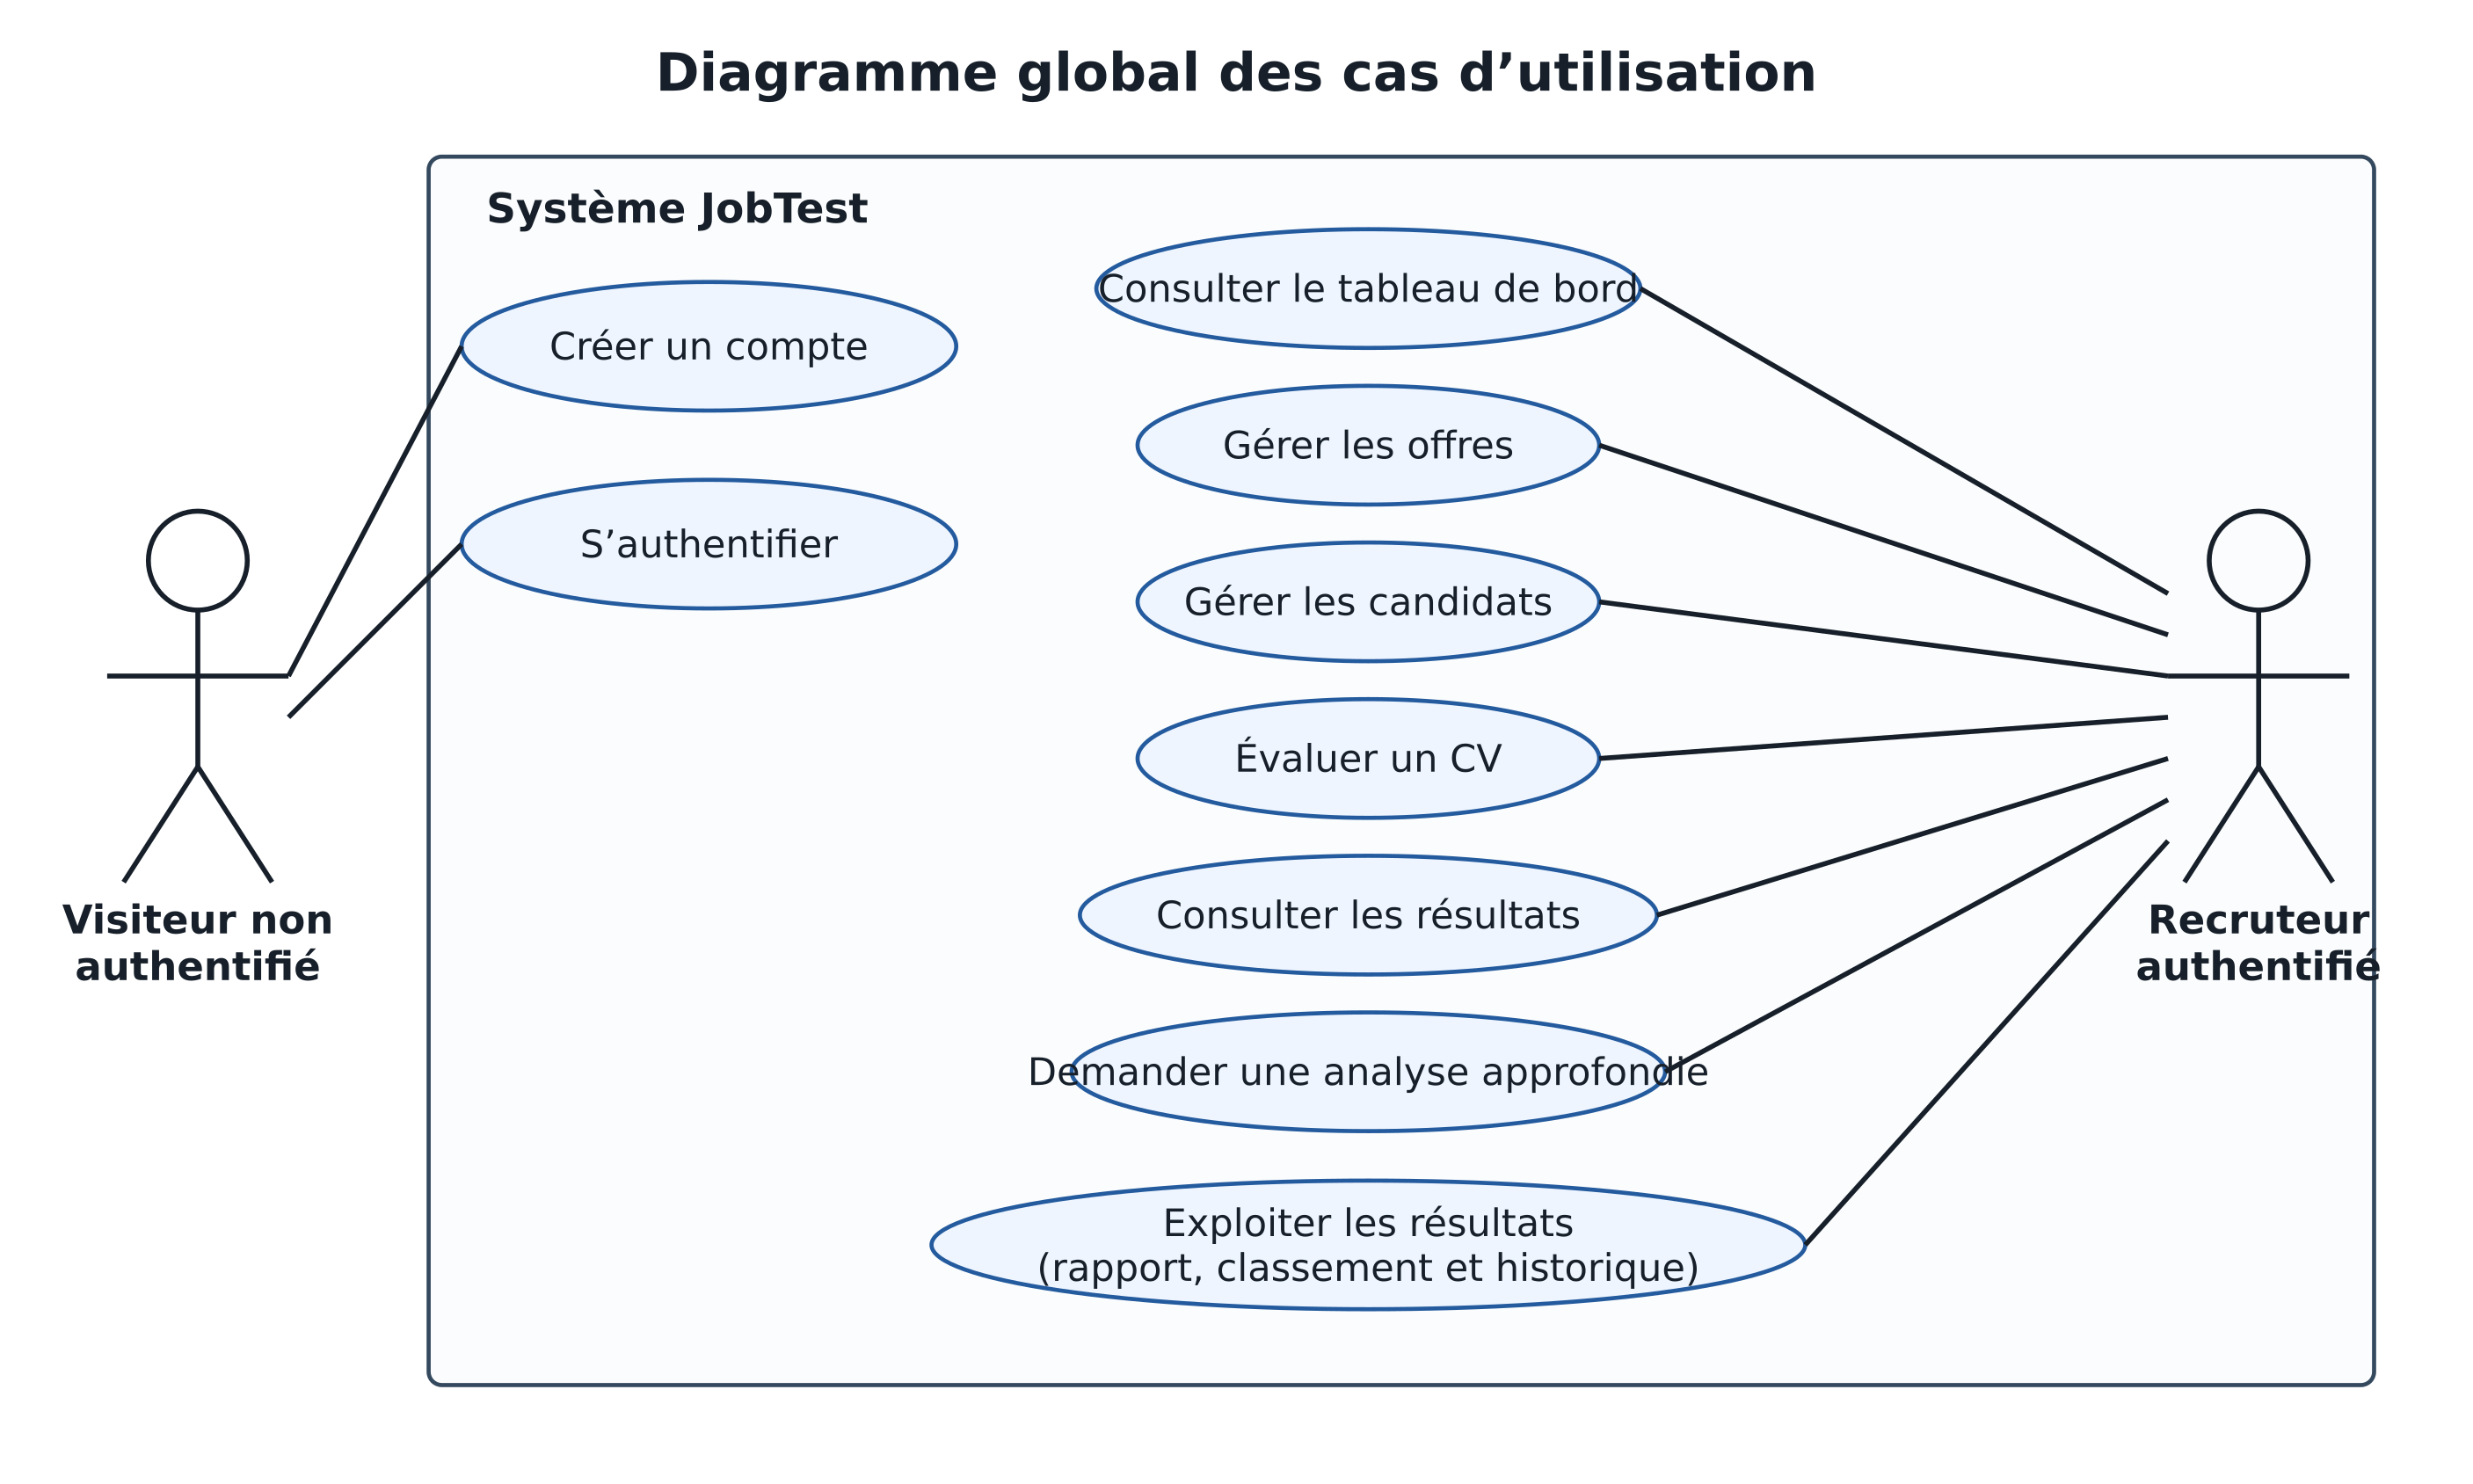
\includegraphics[width=.95\textwidth,height=.76\textheight,keepaspectratio]{img/jobtest_use_cases/01_global.png}
\caption{Diagramme global des cas d'utilisation de JobTest}
\label{fig:uc-global}
\end{figure}

Le visiteur reste limité à la création de compte et à l'authentification. Le recruteur porte tous les cas opérationnels. L'analyse approfondie est une extension facultative de la consultation du résultat ; l'export PDF dépend de l'existence d'un résultat. L'authentification est une précondition aux autres cas et non un lien \textit{include} répété dans tout le diagramme.

\section{Raffinement des cas d'utilisation principaux}
Les diagrammes suivants détaillent les huit parcours significatifs sans transformer les opérations internes en cas d'utilisation. Les relations \textit{include} expriment une sous-action nécessaire au but représenté ; la relation \textit{extend} est réservée à l'analyse approfondie facultative.

La série s'ouvre avec la figure~\ref{fig:uc-auth}, consacrée à l'authentification et à la gestion de session.

\begin{figure}[htbp]\centering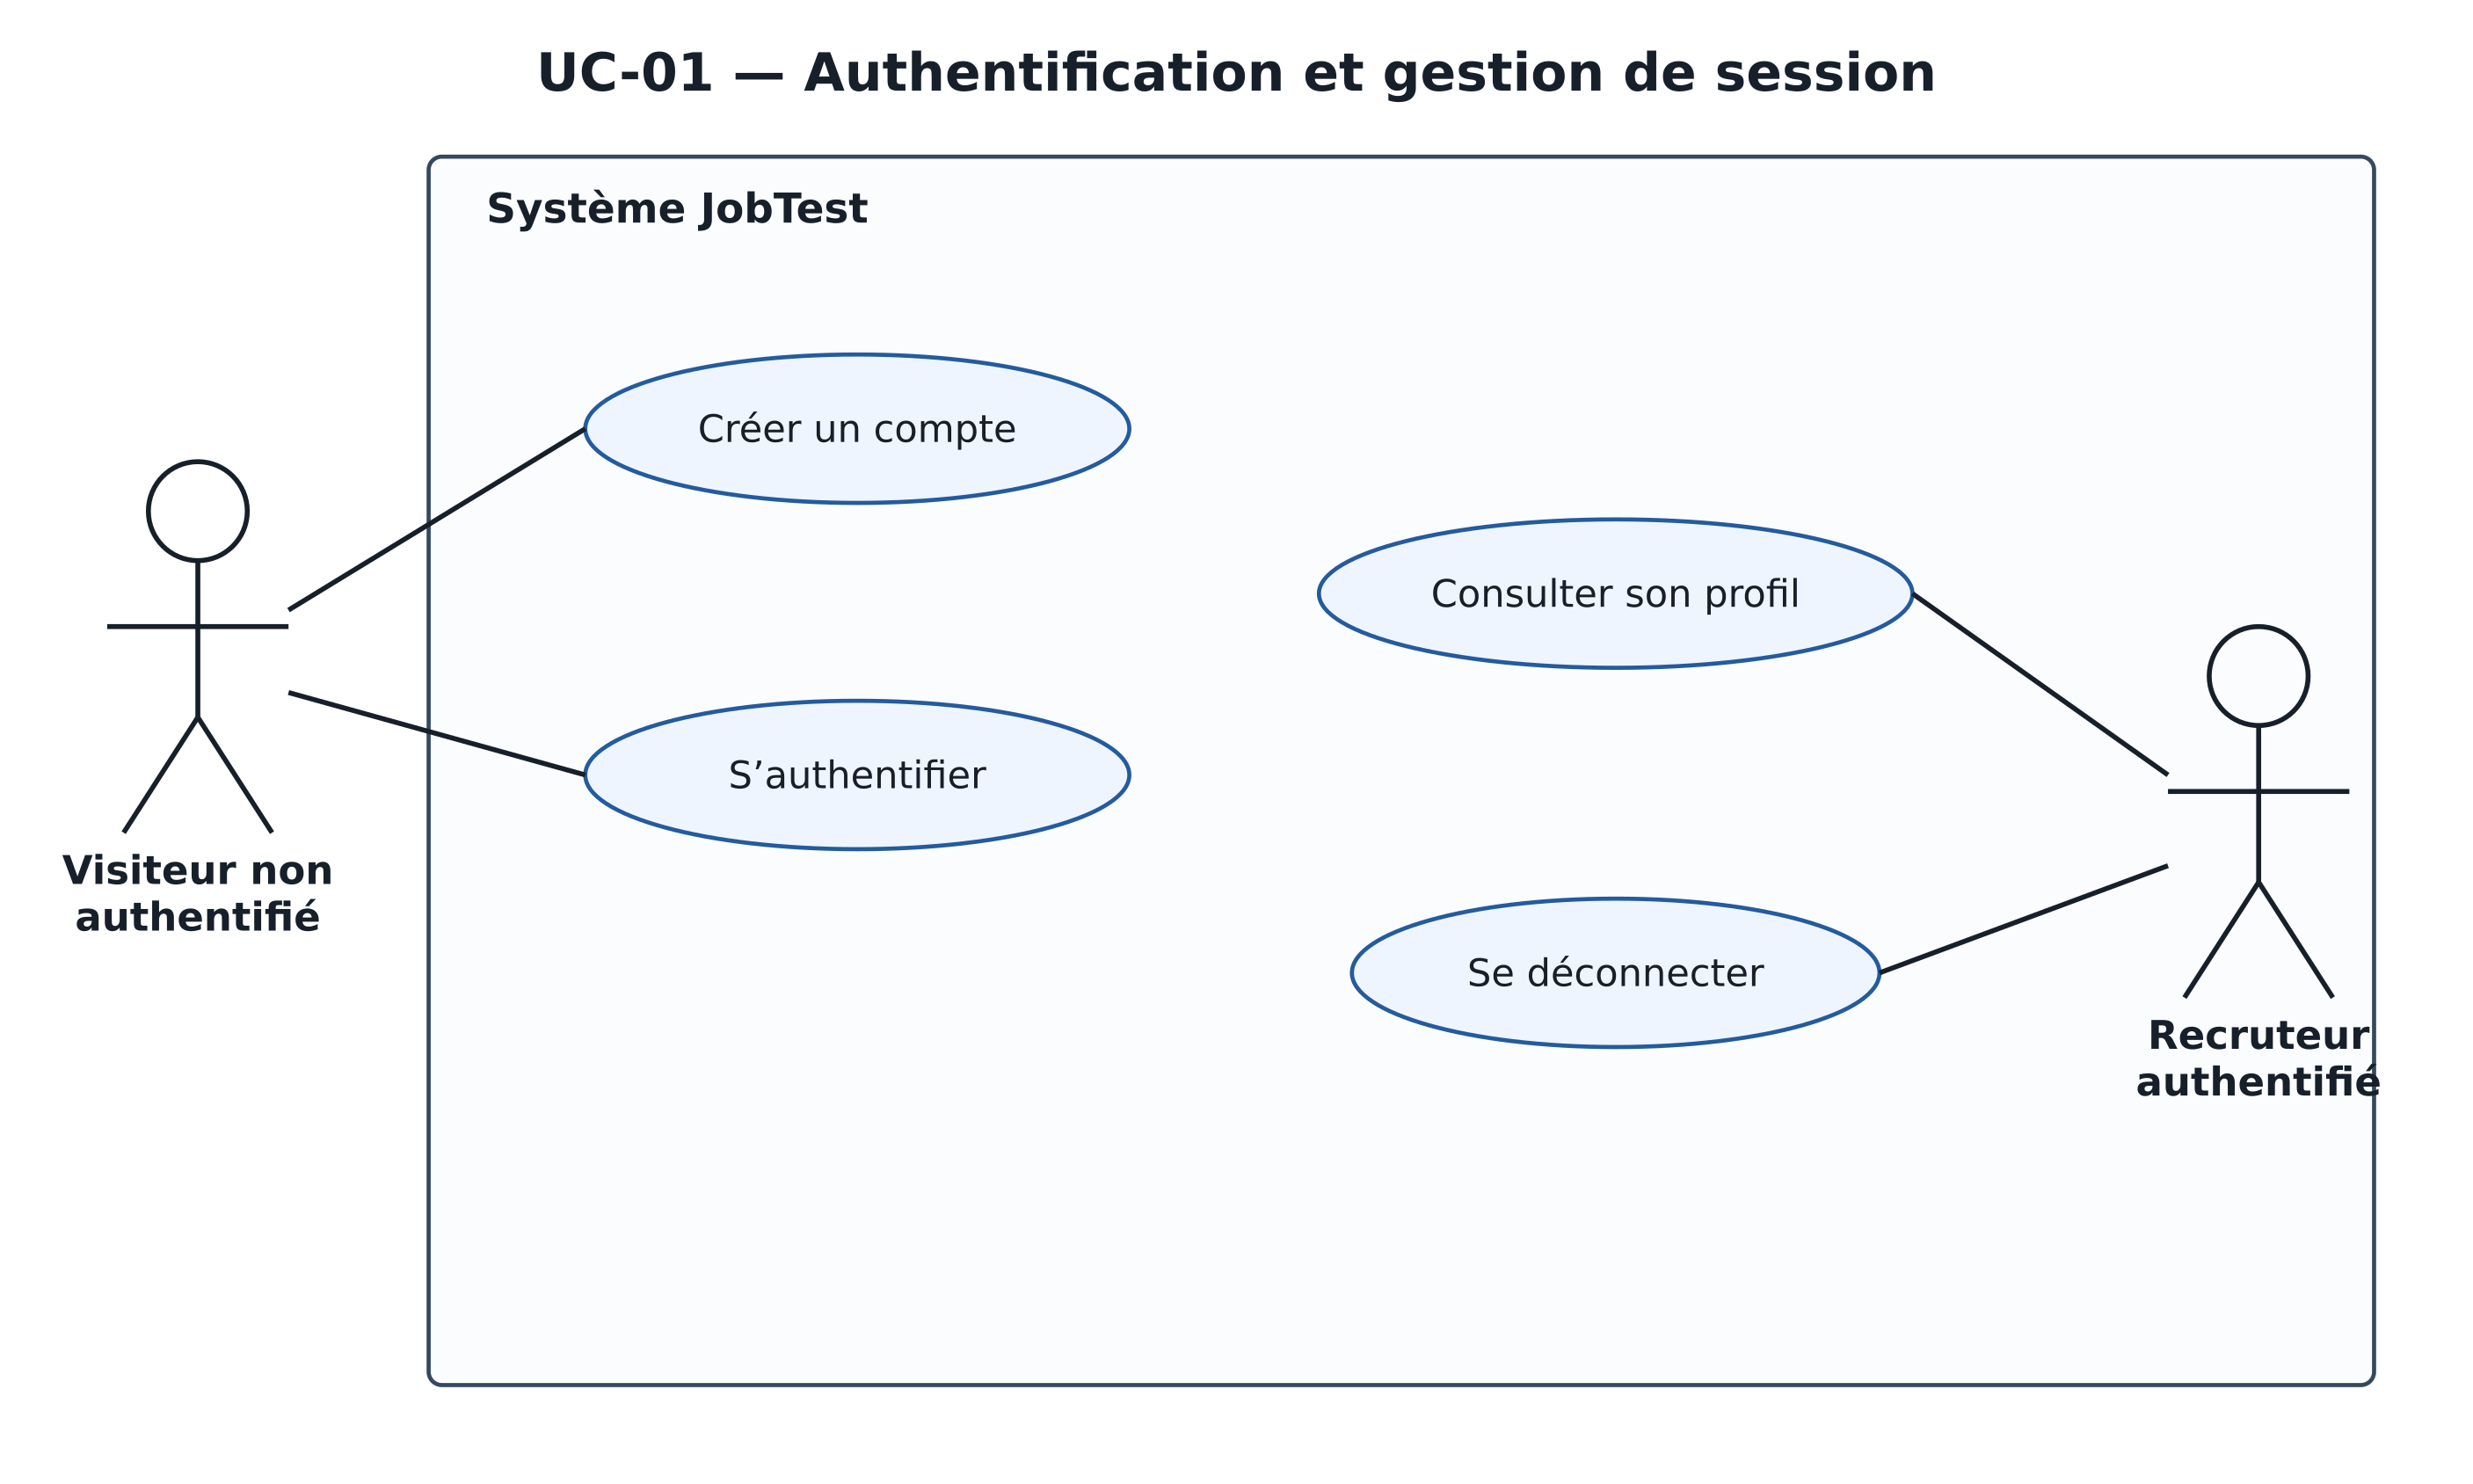
\includegraphics[width=.95\textwidth,height=.76\textheight,keepaspectratio]{img/jobtest_use_cases/02_authentification.png}\caption{UC-01 : authentification et session}\label{fig:uc-auth}\end{figure}
\begin{figure}[htbp]\centering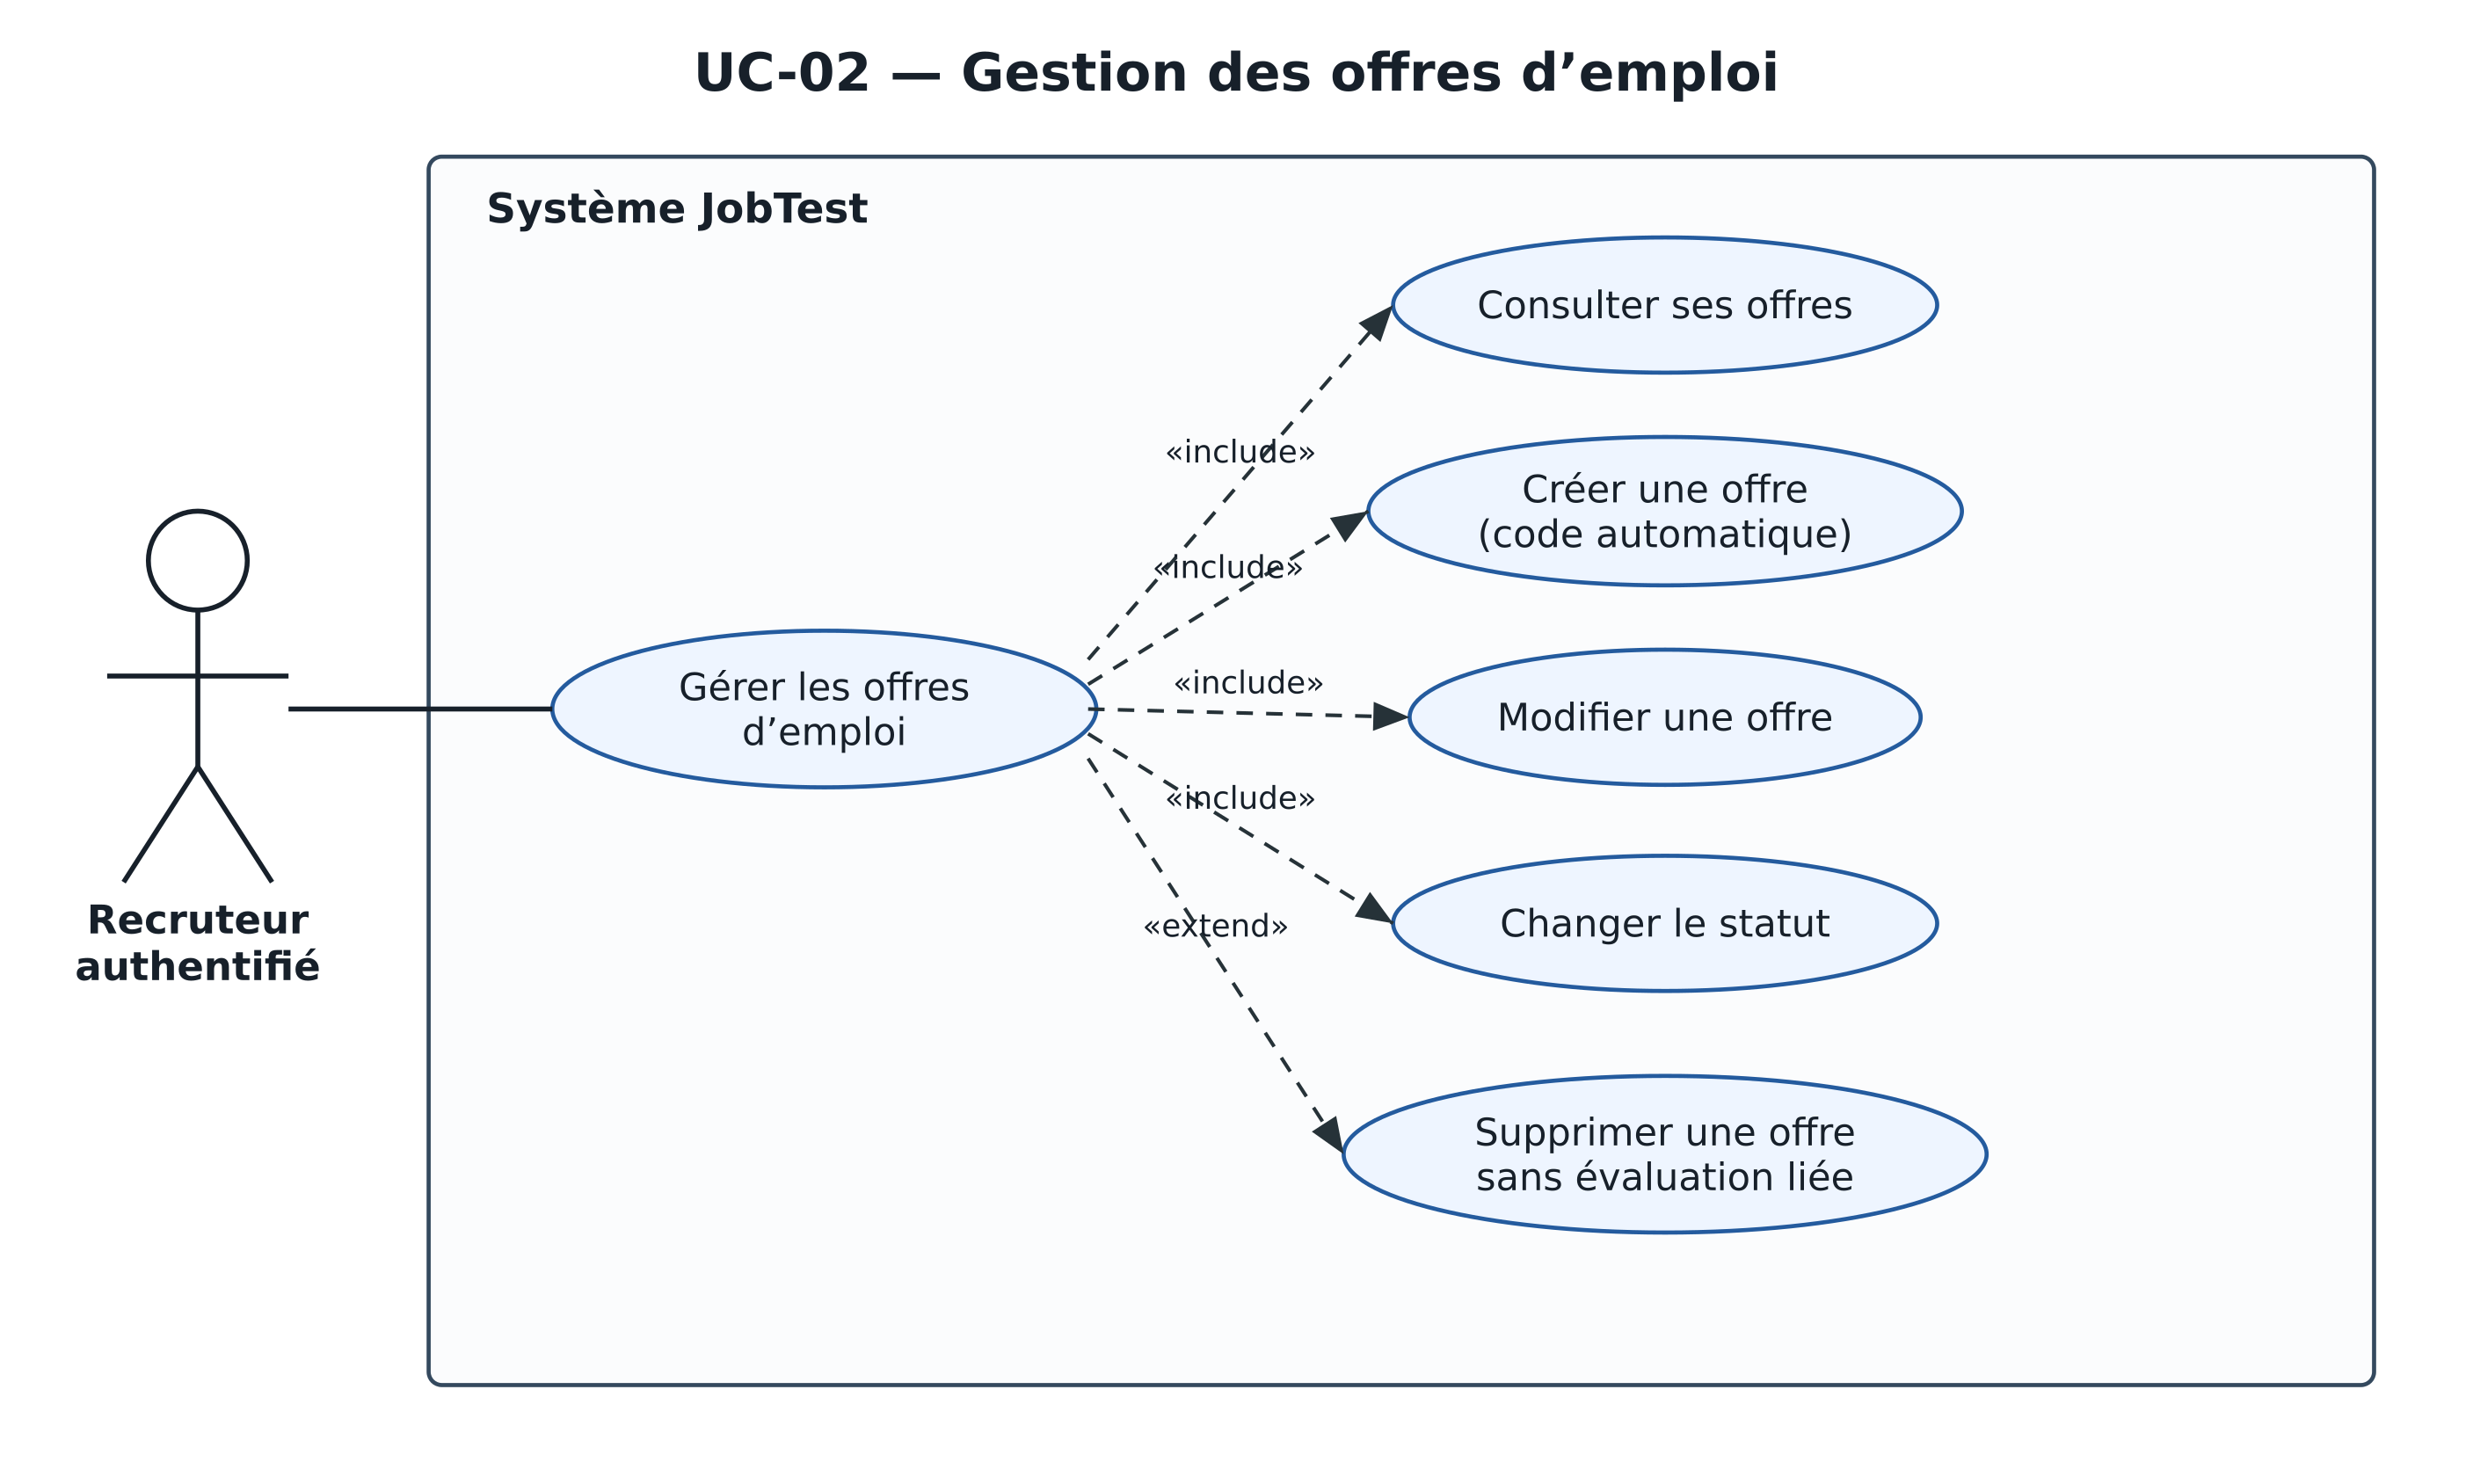
\includegraphics[width=.95\textwidth,height=.76\textheight,keepaspectratio]{img/jobtest_use_cases/03_offres.png}\caption{UC-02 : gestion des offres d'emploi}\label{fig:uc-jobs}\end{figure}
\begin{figure}[htbp]\centering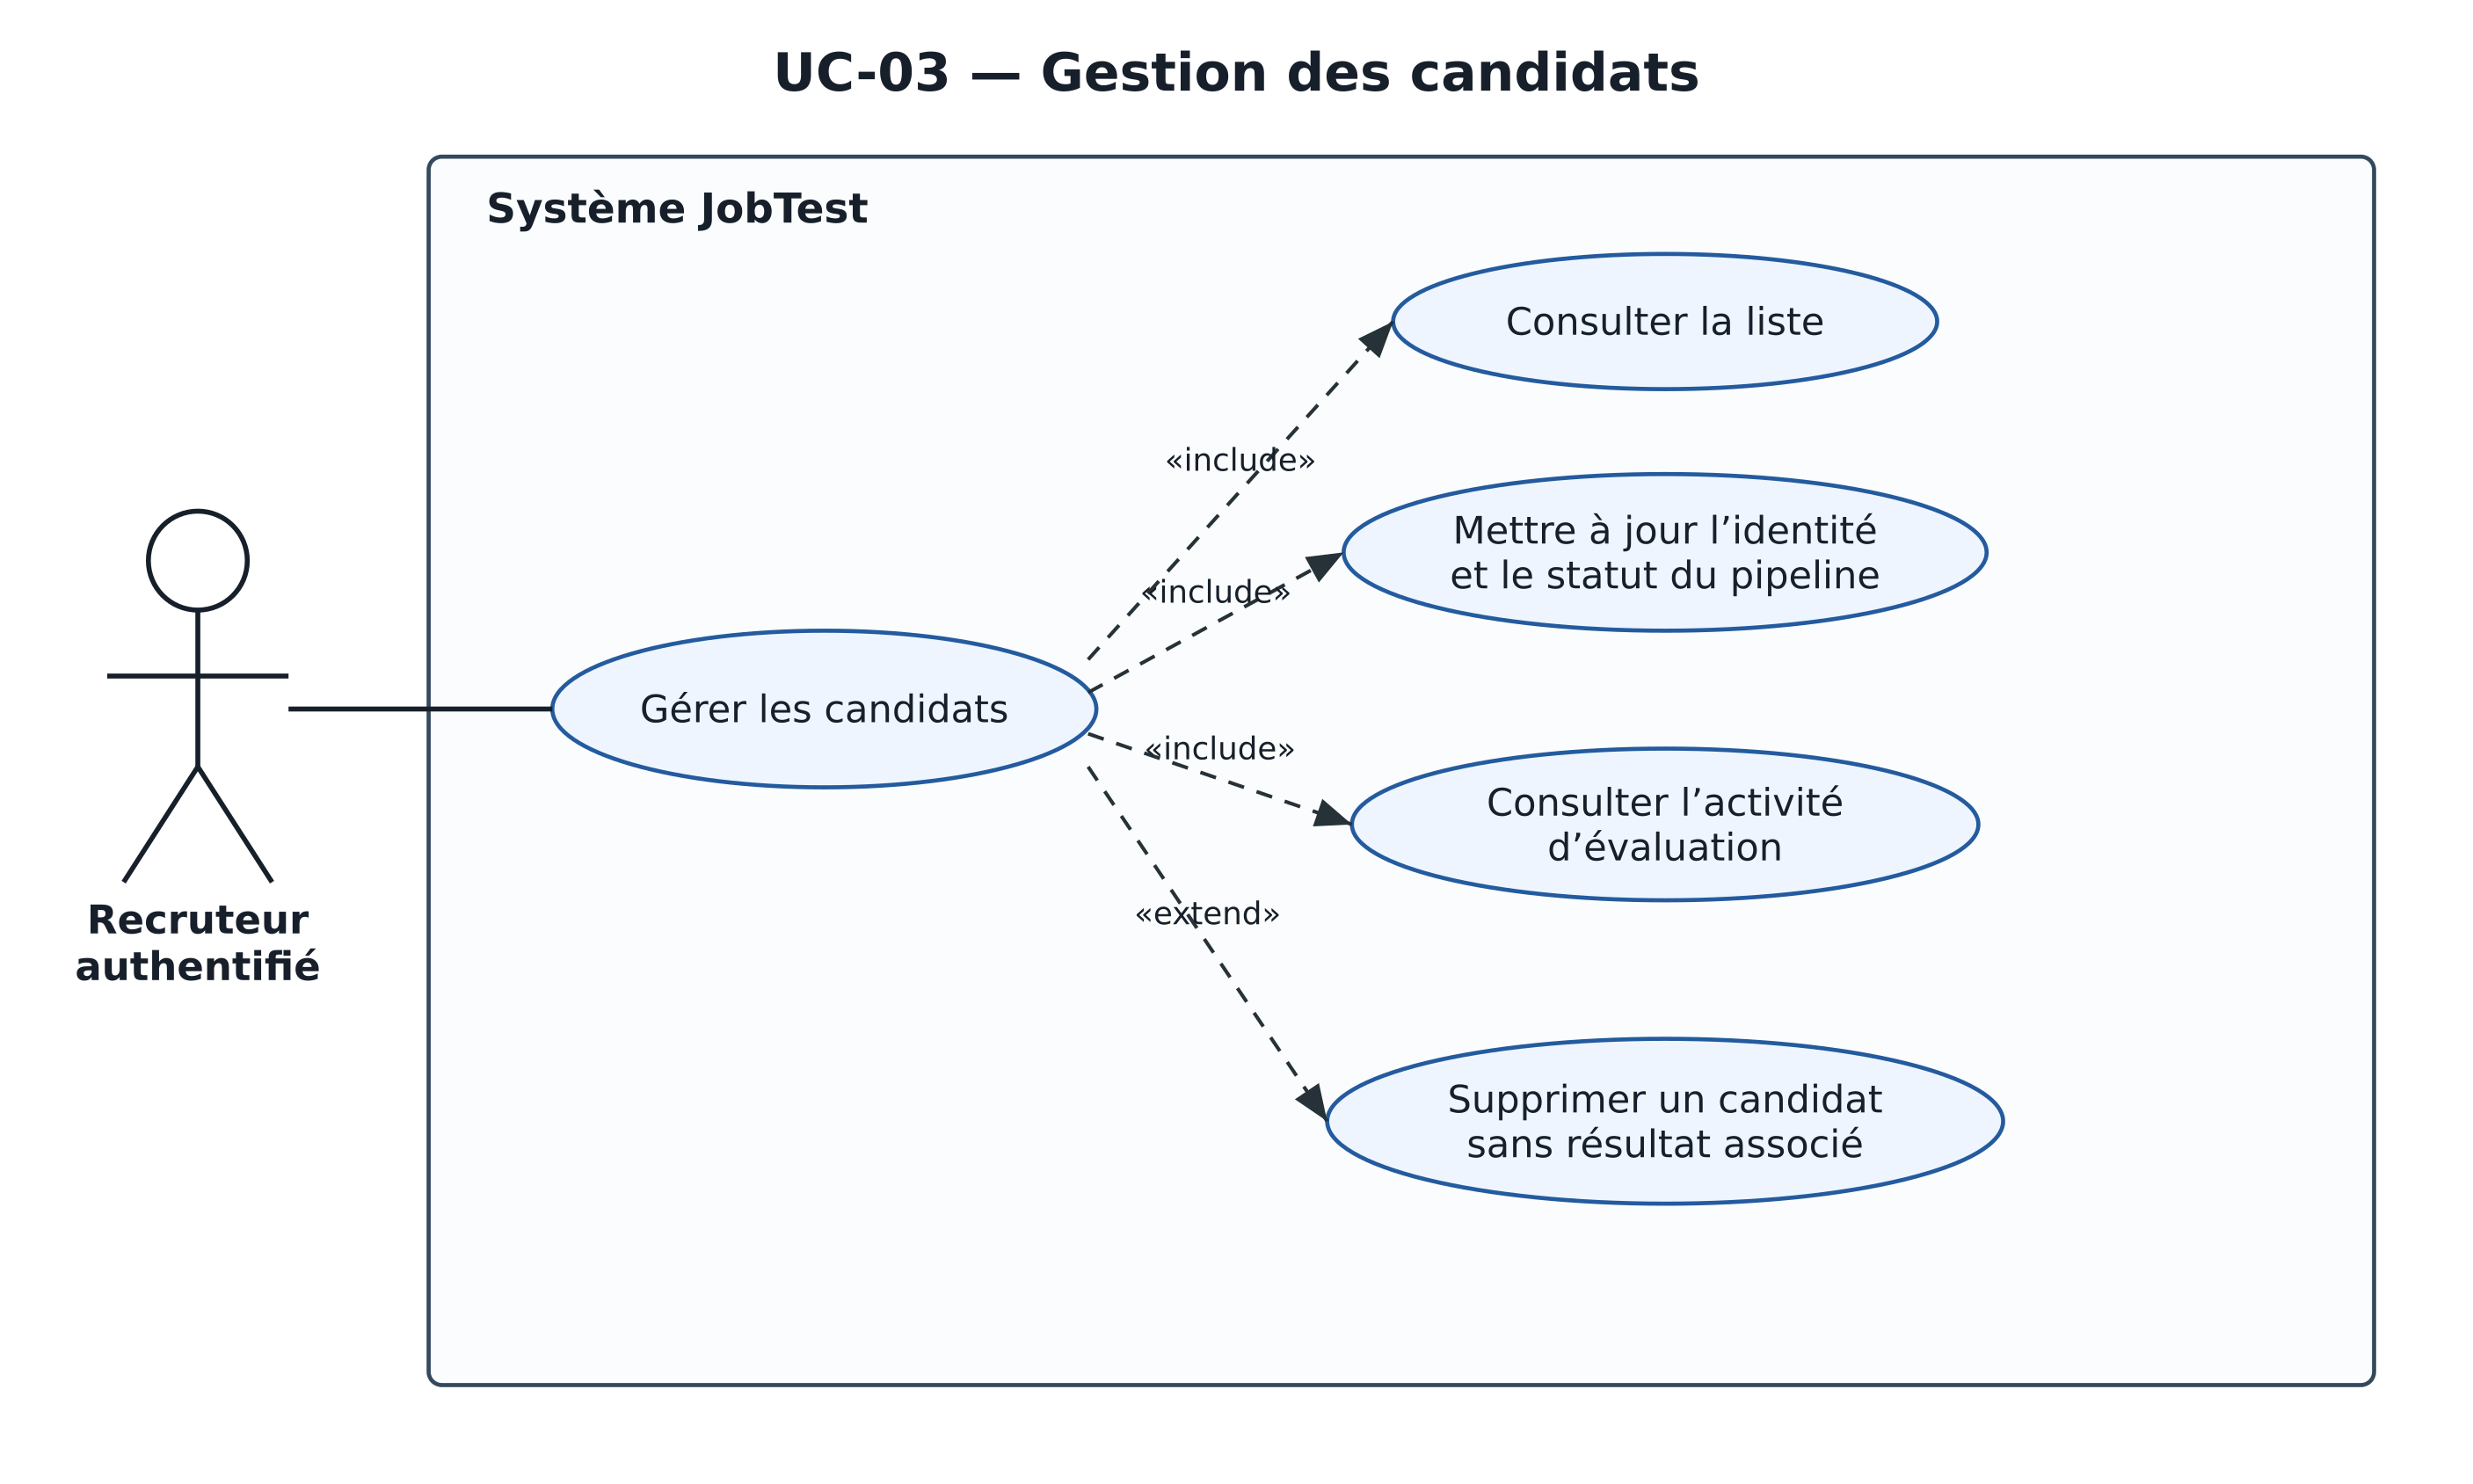
\includegraphics[width=.95\textwidth,height=.76\textheight,keepaspectratio]{img/jobtest_use_cases/04_candidats.png}\caption{UC-03 : gestion des candidats}\label{fig:uc-candidates}\end{figure}
\begin{figure}[htbp]\centering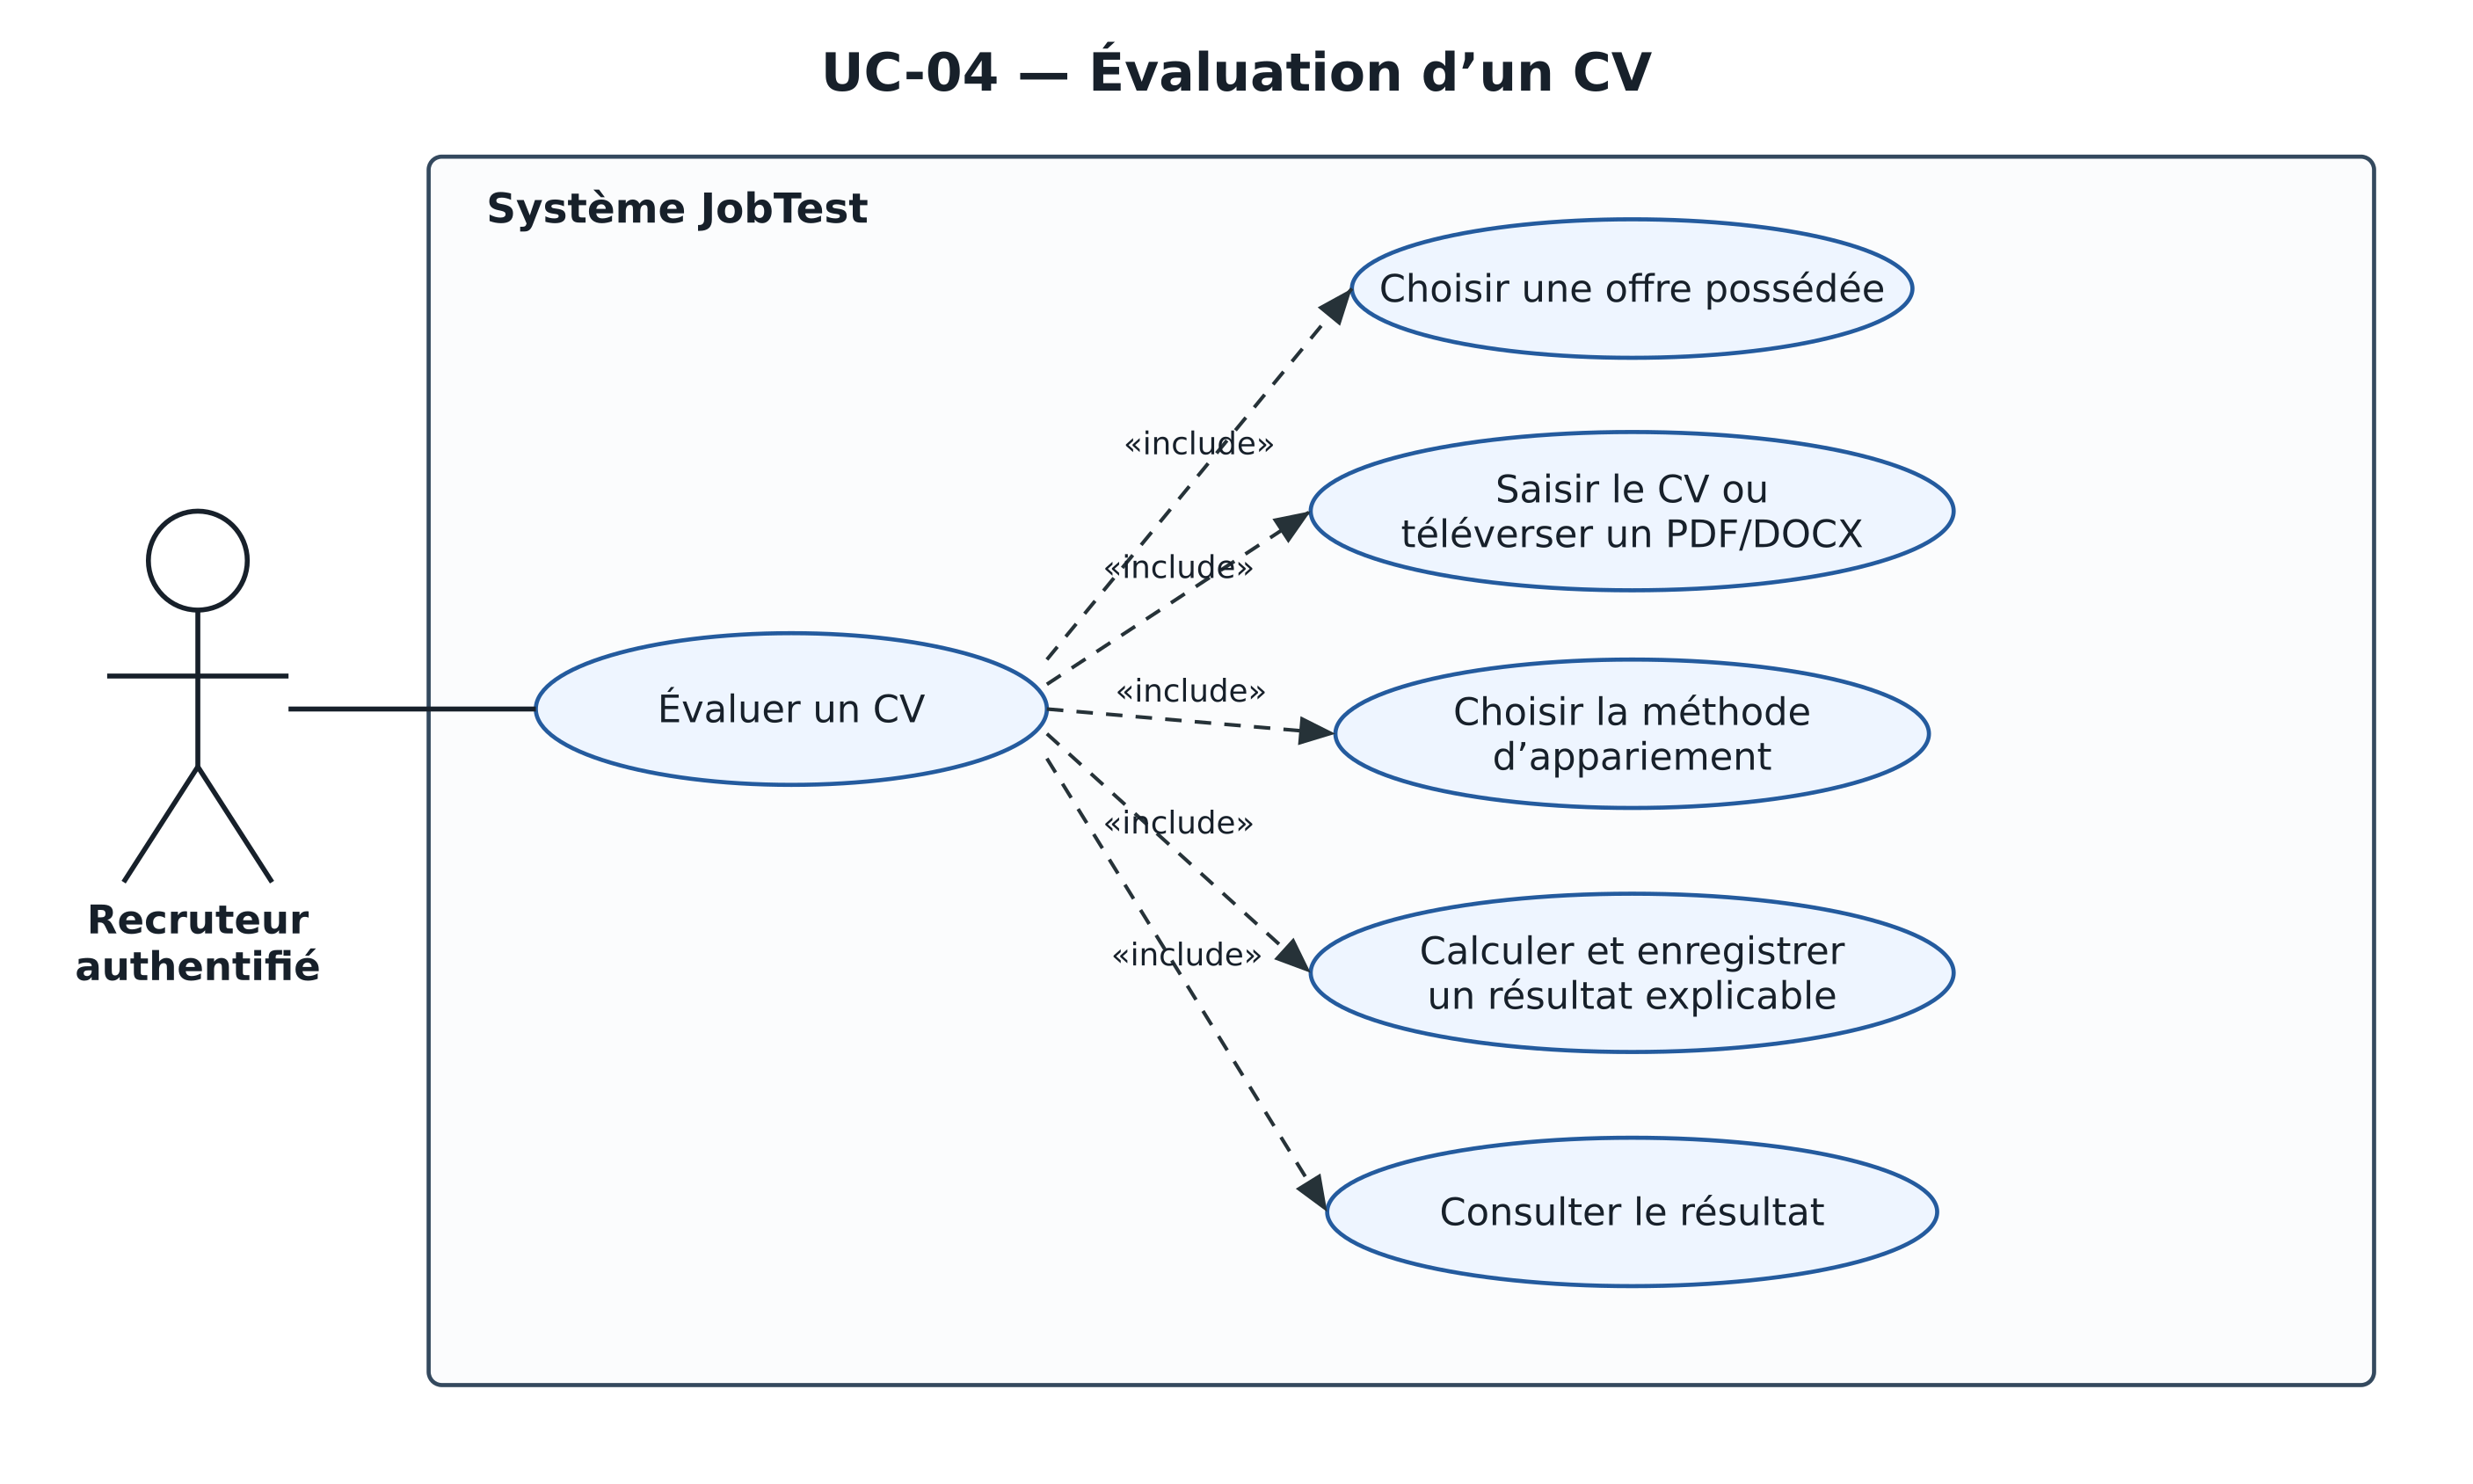
\includegraphics[width=.95\textwidth,height=.76\textheight,keepaspectratio]{img/jobtest_use_cases/05_evaluation_cv.png}\caption{UC-04 : évaluation d'un CV}\label{fig:uc-evaluation}\end{figure}
\begin{figure}[htbp]\centering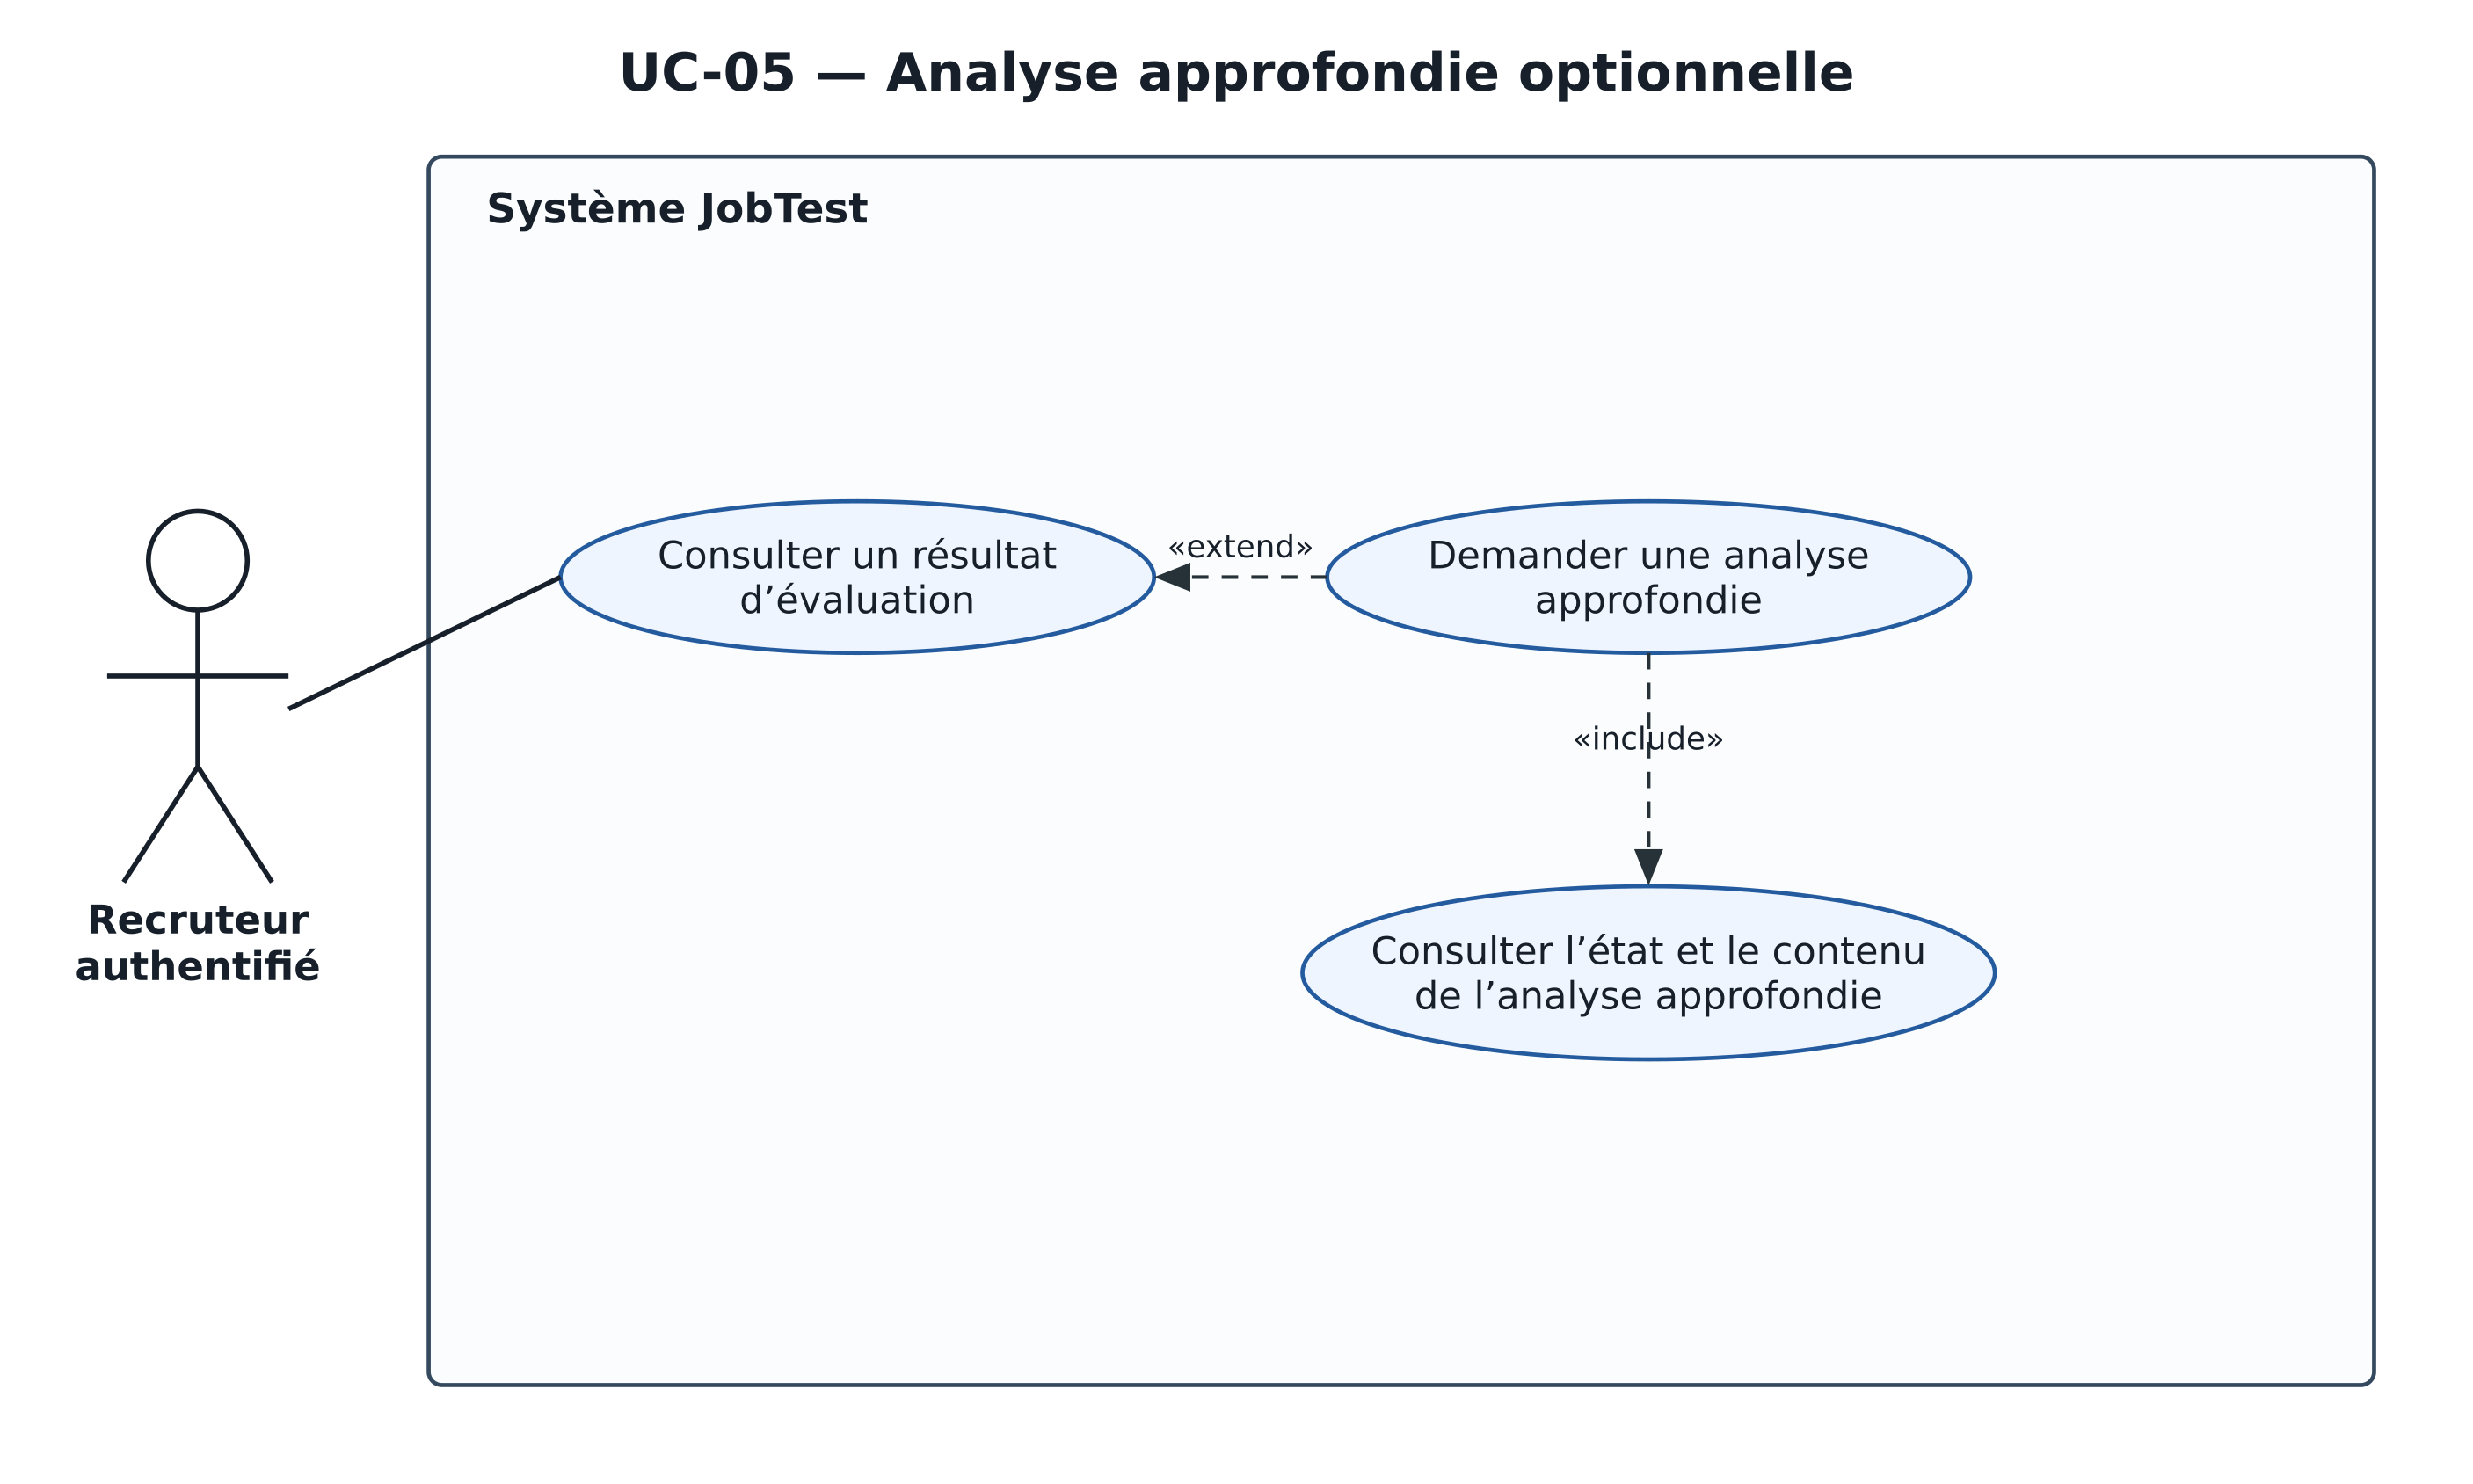
\includegraphics[width=.95\textwidth,height=.76\textheight,keepaspectratio]{img/jobtest_use_cases/06_analyse_approfondie.png}\caption{UC-05 : analyse approfondie optionnelle}\label{fig:uc-deep}\end{figure}
La production du rapport PDF, déclenchée depuis un résultat existant, est représentée par la figure~\ref{fig:uc-report}.

\begin{figure}[htbp]\centering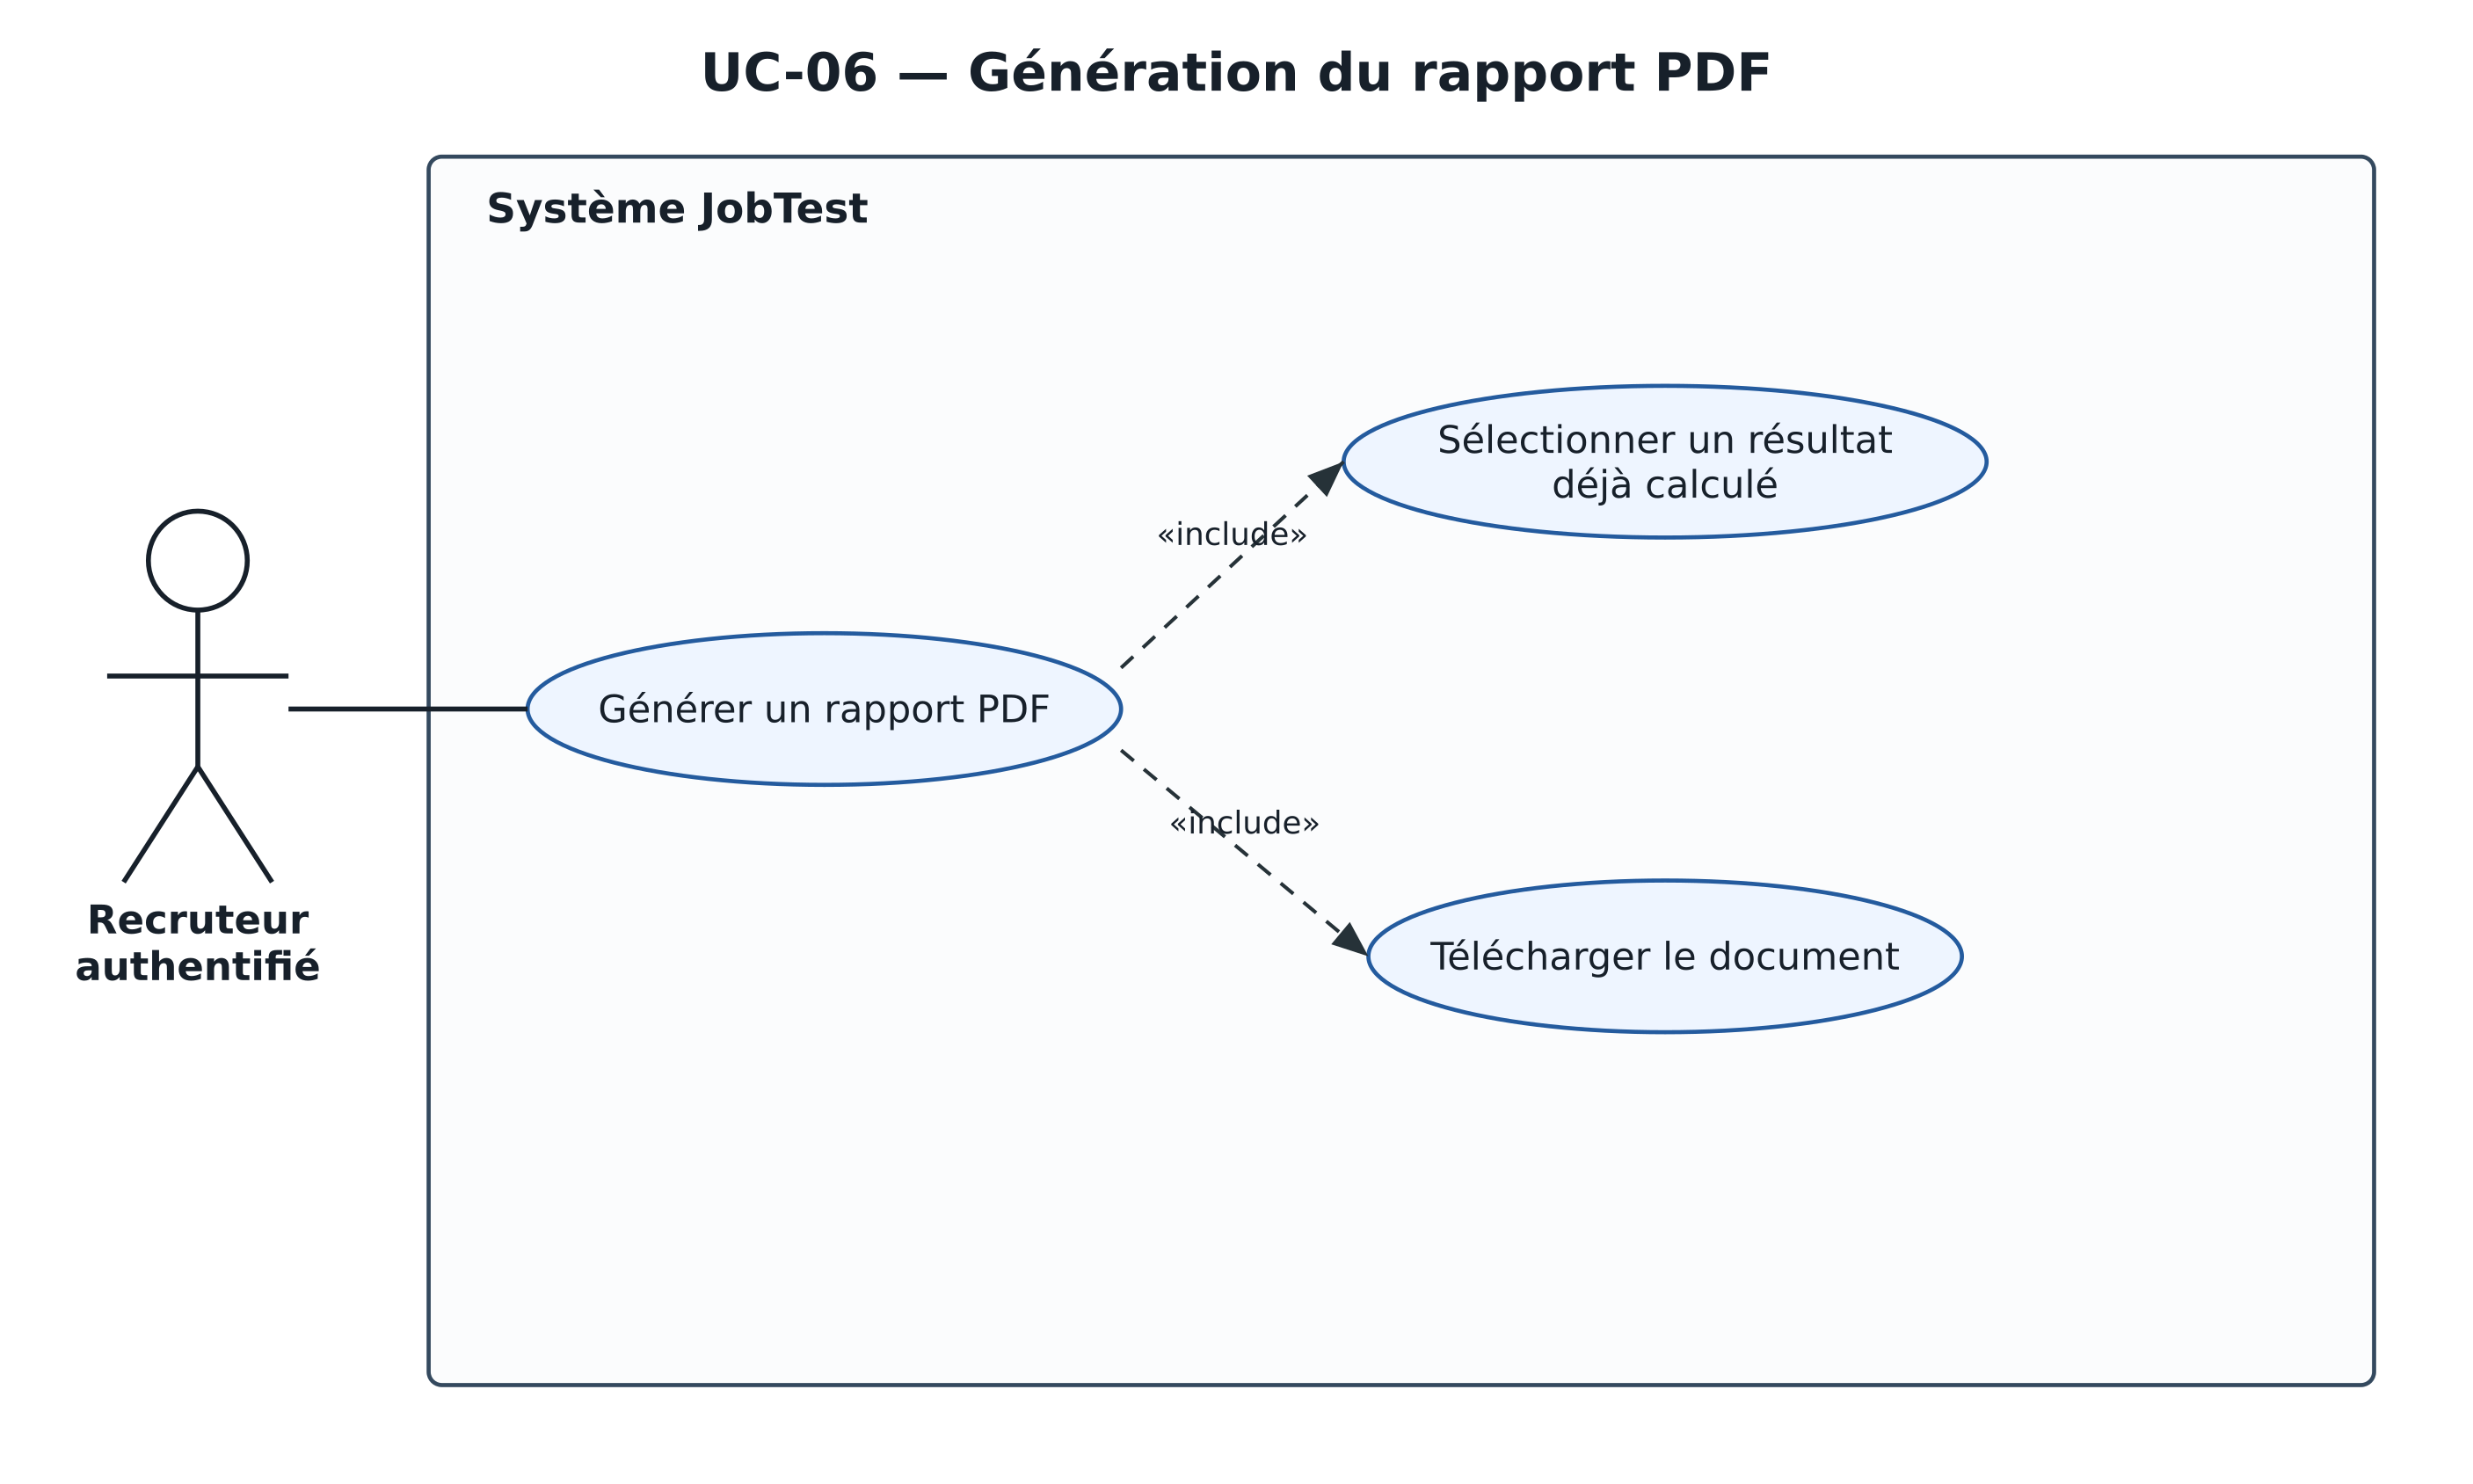
\includegraphics[width=.95\textwidth,height=.76\textheight,keepaspectratio]{img/jobtest_use_cases/07_rapport_pdf.png}\caption{UC-06 : génération du rapport PDF}\label{fig:uc-report}\end{figure}
Le classement de plusieurs candidatures sur une même offre fait l'objet de la figure~\ref{fig:uc-ranking}.

\begin{figure}[htbp]\centering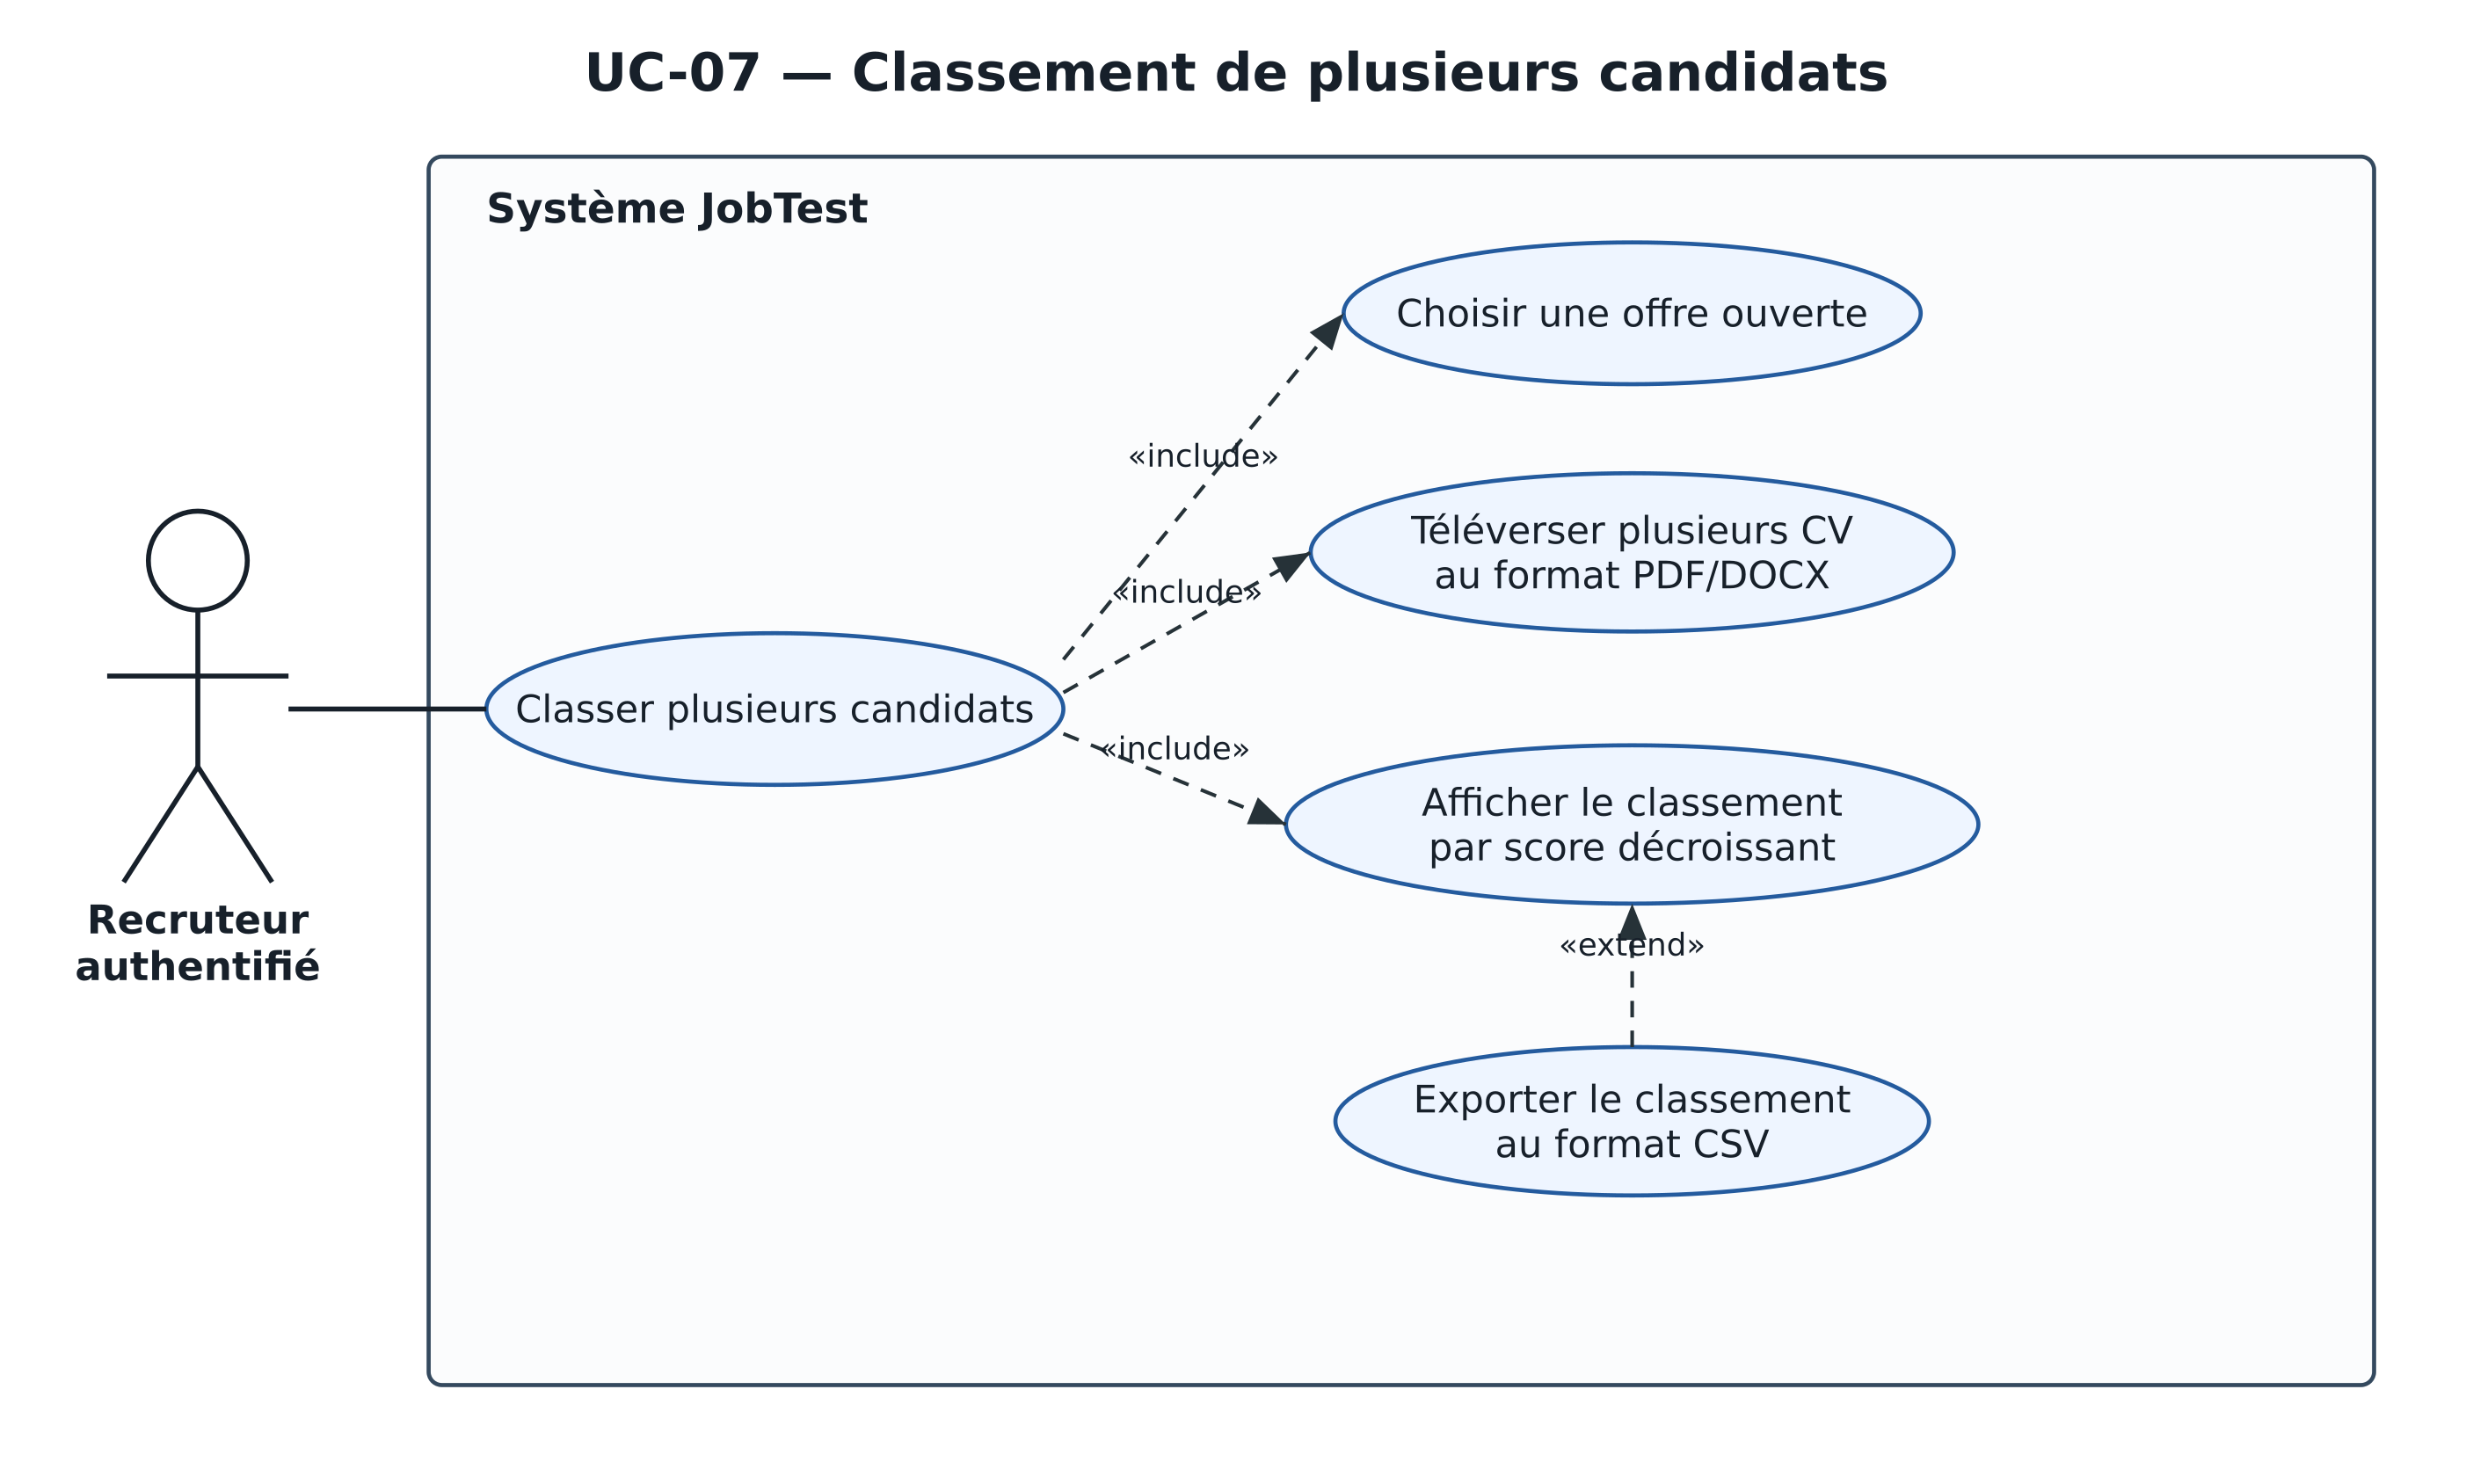
\includegraphics[width=.95\textwidth,height=.76\textheight,keepaspectratio]{img/jobtest_use_cases/08_classement.png}\caption{UC-07 : classement de plusieurs candidats}\label{fig:uc-ranking}\end{figure}
La figure~\ref{fig:uc-history} termine cette série par la consultation de l'historique des évaluations.

\begin{figure}[htbp]\centering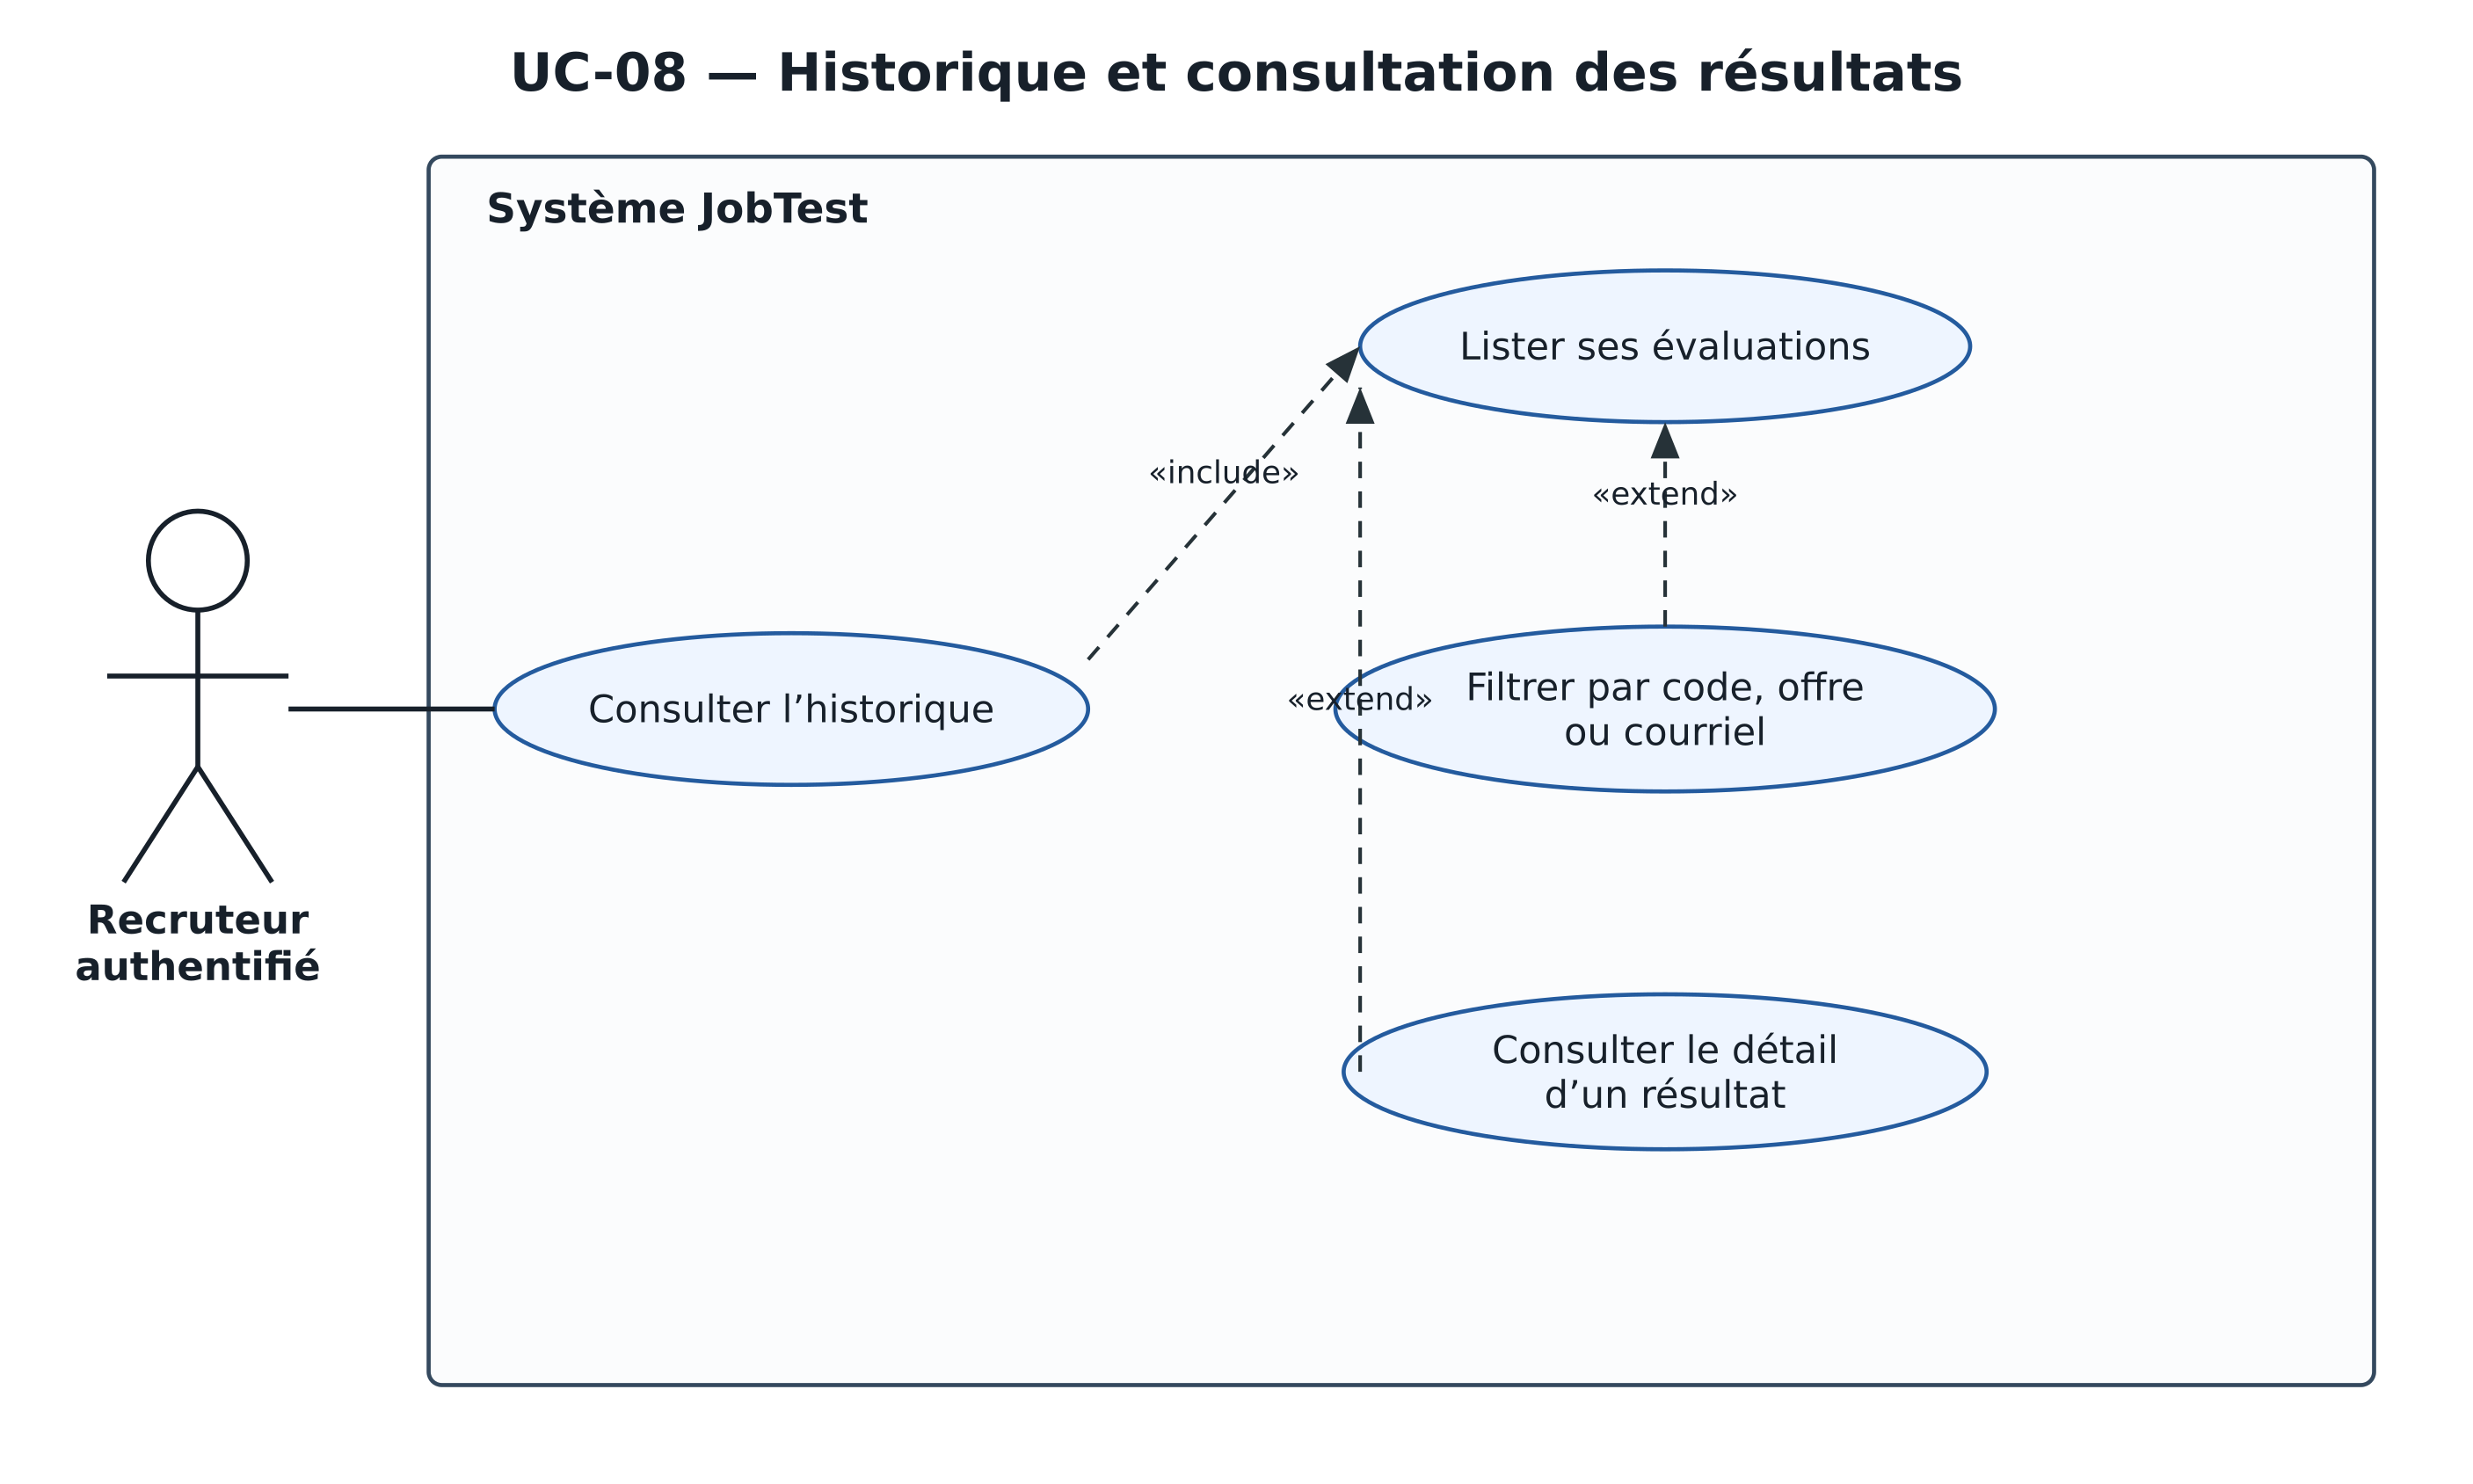
\includegraphics[width=.95\textwidth,height=.76\textheight,keepaspectratio]{img/jobtest_use_cases/09_historique.png}\caption{UC-08 : historique et résultats}\label{fig:uc-history}\end{figure}

Les figures \ref{fig:uc-evaluation} et \ref{fig:uc-deep} isolent explicitement le flux obligatoire d'évaluation du complément LLM. Les figures \ref{fig:uc-jobs} et \ref{fig:uc-candidates} regroupent les opérations CRUD afin de conserver une vue centrée sur le but du recruteur plutôt que sur chaque bouton d'interface.

\clearpage
\section{Descriptions textuelles des cas d'utilisation}
Les huit cas retenus sont maintenant décrits champ par champ, dans le même ordre que les diagrammes précédents. 

Le tableau~\ref{tab:uc01} commence par le cas d'authentification.

\small
\begin{longtable}{|p{3.25cm}|p{11.4cm}|}
\caption{UC-01 : s'authentifier}\label{tab:uc01}\\hline \textbf{Champ} & \textbf{Description}\\hline
Identifiant & UC-01\\ Titre & S'authentifier\\ Acteur principal & Visiteur non authentifié\\ Objectif & Ouvrir une session recruteur donnant accès aux données possédées.\\ Déclencheur & Le visiteur valide le formulaire de connexion.\\ Préconditions & Un compte recruteur existe.\\ Postconditions & Le JWT est stocké côté client et le profil courant est récupérable.\\ Scénario nominal & 1. Le visiteur saisit e-mail et mot de passe. 2. Le système vérifie les identifiants. 3. Le système émet le JWT bearer. 4. L'interface charge \texttt{/auth/me} puis redirige vers l'espace opérationnel.\\ Scénarios alternatifs & Un nouveau visiteur choisit la création de compte, puis revient à la connexion.\\ Exceptions & Identifiants invalides, compte absent ou API indisponible : message d'erreur, aucune session créée.\\ Règles associées & RG-01.\\hline
\end{longtable}

La gestion des offres est décrite dans le tableau~\ref{tab:uc02}.

\begin{longtable}{|p{3.25cm}|p{11.4cm}|}
\caption{UC-02 : gérer une offre d'emploi}\label{tab:uc02}\\hline \textbf{Champ} & \textbf{Description}\\hline
Identifiant & UC-02\\ Titre & Gérer une offre d'emploi\\ Acteur principal & Recruteur authentifié\\ Objectif & Créer, consulter, modifier, clôturer ou supprimer une offre possédée.\\ Déclencheur & Le recruteur ouvre la page des offres ou son formulaire.\\ Préconditions & Session valide.\\ Postconditions & L'offre est créée ou mise à jour ; l'historique associé reste cohérent.\\ Scénario nominal & 1. Le recruteur saisit titre, description, compétences et statut. 2. Le système valide titre et description. 3. À la création, il attribue un code \texttt{JOB-YYYY-NNN}. 4. Il enregistre l'offre sous le recruteur courant. 5. L'interface actualise la liste.\\ Scénarios alternatifs & Le recruteur modifie une offre ou utilise l'action de bascule \texttt{OPEN}/\texttt{CLOSED}.\\ Exceptions & Offre non possédée ou champs obligatoires absents : opération refusée. Suppression avec évaluations : réponse 409 et proposition de clôture.\\ Règles associées & RG-01, RG-02.\\hline
\end{longtable}

Le tableau~\ref{tab:uc03} poursuit avec le suivi des candidats.

\begin{longtable}{|p{3.25cm}|p{11.4cm}|}
\caption{UC-03 : gérer un candidat}\label{tab:uc03}\\hline \textbf{Champ} & \textbf{Description}\\hline
Identifiant & UC-03\\ Titre & Gérer un candidat\\ Acteur principal & Recruteur authentifié\\ Objectif & Mettre à jour et suivre les dossiers candidats issus des évaluations.\\ Déclencheur & Le recruteur consulte la page candidats et choisit un dossier.\\ Préconditions & Session valide ; candidat possédé par le recruteur.\\ Postconditions & Les coordonnées ou le statut de pipeline sont mis à jour, ou le dossier non évalué est supprimé.\\ Scénario nominal & 1. Le système liste les candidats du recruteur. 2. Le recruteur ouvre l'édition. 3. Il modifie nom, e-mail, téléphone ou statut. 4. Le système valide puis enregistre. 5. L'interface affiche les données actualisées.\\ Scénarios alternatifs & Le recruteur consulte l'activité et le meilleur score du dossier.\\ Exceptions & Nom vide, e-mail déjà utilisé ou candidat hors périmètre : mise à jour refusée. Candidat évalué : suppression bloquée.\\ Règles associées & RG-01, RG-03.\\hline
\end{longtable}

Vient ensuite l'évaluation d'un CV, dont le tableau~\ref{tab:uc04} détaille le déroulement et les exceptions.

\begin{longtable}{|p{3.25cm}|p{11.4cm}|}
\caption{UC-04 : évaluer un CV}\label{tab:uc04}\\hline \textbf{Champ} & \textbf{Description}\\hline
Identifiant & UC-04\\ Titre & Évaluer un CV\\ Acteur principal & Recruteur authentifié\\ Objectif & Obtenir et conserver une évaluation explicable d'un CV contre une offre.\\ Déclencheur & Le recruteur lance l'évaluation depuis la page d'analyse.\\ Préconditions & Session valide ; offre possédée ; texte de CV ou fichier PDF/DOCX disponible ; seuils valides.\\ Postconditions & Un \texttt{MatchResult} est persisté avec score, décision, explication et métadonnées.\\ Scénario nominal & 1. Le recruteur choisit une offre. 2. Il fournit identité facultative et texte CV, ou un PDF/DOCX. 3. Le système valide l'entrée et extrait le texte si nécessaire. 4. Il exécute l'appariement statistique choisi. 5. Le \textit{DecisionEngine} détermine le verdict. 6. Le système persiste le résultat. 7. L'interface affiche score, sous-scores, compétences, écarts et recommandations.\\ Scénarios alternatifs & Le recruteur choisit l'une des méthodes admises : hybride, embedding, TF-IDF ou compétences.\\ Exceptions & Offre manquante ; texte inférieur à cinq mots ; format non admis ; document sans texte lisible ; seuils invalides ; erreur de persistance : aucune évaluation valide n'est affichée comme réussie.\\ Règles associées & RG-01, RG-04, RG-05, RG-09, RG-10.\\hline
\end{longtable}

Le tableau~\ref{tab:uc05} traite la demande d'analyse approfondie et son caractère facultatif.

\begin{longtable}{|p{3.25cm}|p{11.4cm}|}
\caption{UC-05 : demander une analyse approfondie}\label{tab:uc05}\\hline \textbf{Champ} & \textbf{Description}\\hline
Identifiant & UC-05\\ Titre & Demander une analyse approfondie\\ Acteur principal & Recruteur authentifié\\ Objectif & Compléter un résultat persistant par une lecture qualitative locale.\\ Déclencheur & Le résultat Layer 1 est déjà affiché et le recruteur demande l'analyse.\\ Préconditions & Session valide ; \texttt{MatchResult} possédé par le recruteur.\\ Postconditions & Une enveloppe LLM est affichée ; elle est sauvegardée seulement si son état est \texttt{ok}.\\ Scénario nominal & 1. Le recruteur demande l'analyse. 2. Le système reconstruit le contexte depuis le résultat existant. 3. Il sollicite Ollama. 4. Il vérifie la réponse. 5. Il affiche la synthèse et persiste l'enveloppe réussie.\\ Scénarios alternatifs & Une analyse déjà disponible peut être relue dans le résultat conservé.\\ Exceptions & LLM désactivé, indisponible, sortie malformée ou incohérente : l'état est retourné sans modifier score ni verdict.\\ Règles associées & RG-01, RG-06, RG-08.\\hline
\end{longtable}

La génération du rapport est reprise par le tableau~\ref{tab:uc06}.

\begin{longtable}{|p{3.25cm}|p{11.4cm}|}
\caption{UC-06 : générer un rapport PDF}\label{tab:uc06}\\hline \textbf{Champ} & \textbf{Description}\\hline
Identifiant & UC-06\\ Titre & Générer un rapport PDF\\ Acteur principal & Recruteur authentifié\\ Objectif & Télécharger une restitution portable d'une évaluation calculée.\\ Déclencheur & Le recruteur active l'export depuis le résultat.\\ Préconditions & Un résultat et son explication sont disponibles.\\ Postconditions & Le navigateur reçoit le PDF ; aucun nouveau score n'est calculé.\\ Scénario nominal & 1. Le recruteur sélectionne l'export. 2. L'interface transmet le résultat, l'explication, les recommandations et les libellés disponibles. 3. Le système produit le document. 4. Le navigateur déclenche le téléchargement.\\ Scénarios alternatifs & Le recruteur revient au résultat sans exporter.\\ Exceptions & Données de résultat incomplètes ou échec de génération : l'interface signale l'échec.\\ Règles associées & RG-01, RG-09.\\hline
\end{longtable}

Le tableau~\ref{tab:uc07} formalise le classement de plusieurs candidats pour une offre unique.

\begin{longtable}{|p{3.25cm}|p{11.4cm}|}
\caption{UC-07 : classer plusieurs candidats}\label{tab:uc07}\\hline \textbf{Champ} & \textbf{Description}\\hline
Identifiant & UC-07\\ Titre & Classer plusieurs candidats\\ Acteur principal & Recruteur authentifié\\ Objectif & Comparer plusieurs CV contre une seule offre.\\ Déclencheur & Le recruteur sélectionne une offre et plusieurs fichiers.\\ Préconditions & Session valide ; offre ouverte disponible ; fichiers PDF/DOCX lisibles.\\ Postconditions & Chaque évaluation réussie est persistée et l'interface affiche le classement décroissant.\\ Scénario nominal & 1. Le recruteur choisit une offre. 2. Il ajoute plusieurs CV PDF/DOCX. 3. L'interface soumet chaque fichier au flux d'évaluation. 4. Elle collecte les résultats réussis. 5. Elle les trie par score décroissant. 6. Elle permet l'export CSV du classement courant.\\ Scénarios alternatifs & Le recruteur retire un fichier avant le lancement.\\ Exceptions & Aucun poste, fichier non lisible ou évaluation en échec : le fichier concerné est signalé ; les autres résultats valides restent consultables.\\ Règles associées & RG-01, RG-04, RG-05, RG-10.\\hline
\end{longtable}

La consultation de l'historique clôt la série avec le tableau~\ref{tab:uc08}.

\begin{longtable}{|p{3.25cm}|p{11.4cm}|}
\caption{UC-08 : consulter l'historique}\label{tab:uc08}\\hline \textbf{Champ} & \textbf{Description}\\hline
Identifiant & UC-08\\ Titre & Consulter l'historique et les résultats\\ Acteur principal & Recruteur authentifié\\ Objectif & Retrouver les évaluations persistées et leur détail.\\ Déclencheur & Le recruteur ouvre la page historique.\\ Préconditions & Session valide.\\ Postconditions & Une liste filtrée ou le détail d'un résultat possédé est affiché.\\ Scénario nominal & 1. Le système liste les évaluations du recruteur par date décroissante. 2. Le recruteur filtre par code, offre ou e-mail. 3. Il sélectionne une ligne. 4. Le système vérifie l'appartenance et retourne le détail. 5. L'interface affiche les métadonnées et données associées.\\ Scénarios alternatifs & Le recruteur consulte l'historique sans filtre ou revient à la liste.\\ Exceptions & Identifiant absent ou résultat d'un autre recruteur : accès refusé ; erreur réseau : état d'erreur affiché.\\ Règles associées & RG-01, RG-09.\\hline
\end{longtable}
\normalsize

\section{Matrice de traçabilité}
La matrice relie les besoins aux cas d'utilisation et à des groupes de routes ou composants observés. Elle ne remplace pas une documentation API exhaustive ; elle constitue une preuve de correspondance entre l'analyse et la version implémentée.

Le tableau~\ref{tab:tracabilite} en présente le contenu.

{\footnotesize\setlength{\tabcolsep}{2pt}
\begin{longtable}{|>{\raggedright\arraybackslash\scriptsize}p{2.05cm}|>{\raggedright\arraybackslash}p{1.95cm}|>{\raggedright\arraybackslash}p{4.4cm}|>{\raggedright\arraybackslash}p{4.55cm}|}
\caption{Matrice de traçabilité des besoins}\label{tab:tracabilite}\\
\hline \textbf{Besoin} & \textbf{Cas d'utilisation} & \textbf{Composant ou route vérifiée} & \textbf{Critère de validation}\\ \hline
\endfirsthead
\hline \textbf{Besoin} & \textbf{Cas d'utilisation} & \textbf{Composant ou route vérifiée} & \textbf{Critère de validation}\\ \hline
\endhead
BF-AUTH-01--03 & UC-01 & \texttt{/auth/register}, \texttt{/auth/login}, \texttt{/auth/me}, client API & Compte créé, jeton reçu, profil chargé et jeton effacé à la déconnexion.\\
\hline
BF-JOB-01--04 & UC-02 & \texttt{/ui/job-offers}, page \texttt{/jobs} & Création codée, mise à jour, statuts et garde 409 vérifiables.\\
\hline
BF-CAND-01--03 & UC-03 & \texttt{/ui/candidates}, page \texttt{/candidates} & Liste propriétaire, édition de pipeline et suppression conditionnelle.\\
\hline
BF-EVAL-01--03 & UC-04 & \texttt{/ui/evaluate}, \texttt{/ui/evaluate/file}, \texttt{evaluate\_and\_persist} & Résultat persistant et explication après texte ou fichier valide.\\
\hline
BF-LLM-01 & UC-05 & \texttt{/ui/evaluate/deep-analysis}, \texttt{llm\_reasoning} & États LLM rendus sans changement du verdict.\\
\hline
BF-REPORT-01 & UC-06 & \texttt{/report/pdf}, client \texttt{reportPdf} & Réponse PDF téléchargeable depuis le résultat.\\
\hline
BF-RANK-01--02 & UC-07 & page \texttt{/leaderboard}, \texttt{evaluateFile} & Tri décroissant des résultats et CSV côté client.\\
\hline
BF-HIST-01 & UC-08 & \texttt{/ui/matches}, \texttt{/ui/matches/\{id\}}, page \texttt{/history} & Liste filtrée et détail soumis à l'appartenance.\\
\hline
BF-QUALITY-01--02 & UC global & \texttt{/ui/compare}, \texttt{/ui/quality} & Comparaison sans persistance et benchmark file-backed distingués.\\
\hline
BF-SETTINGS-01 & UC global & \texttt{decision-config.tsx}, page \texttt{/settings} & Seuils validés, envoyés aux nouvelles évaluations et mémorisés avec elles.\\
\hline
\end{longtable}\par}
\normalsize

\section{Contraintes et hypothèses}
Le tableau~\ref{tab:contraintes-jobtest} rassemble ces contraintes et hypothèses ainsi que leur effet sur l'analyse.

\begin{table}[htbp]
\centering\small
\begin{tabularx}{\textwidth}{|p{3.3cm}|p{4.1cm}|X|}
\hline
\textbf{Nature} & \textbf{Contrainte ou hypothèse} & \textbf{Effet sur l'analyse}\\
\hline
Fonctionnelle & Aucun portail candidat ni décision autonome d'embauche. & Le recruteur reste l'acteur opérationnel et décideur final.\\
\hline
Fonctionnelle & Les paramètres de seuil sont locaux à la session du navigateur. & Ils ne constituent pas une politique serveur globale et n'écrasent pas l'historique.\\
\hline
Technique & Textes de CV et d'offres possibles en français ou anglais. & La qualité dépend du contenu extrait et des modèles disponibles.\\
\hline
Technique & PDF/DOCX seulement ; extraction parfois impossible ou incomplète. & Les fichiers non lisibles sont rejetés avant évaluation.\\
\hline
Technique & Ollama local, CPU/RAM limités et latence notable. & La Deep Analysis est optionnelle, séparée du verdict et susceptible d'indisponibilité.\\
\hline
Évaluation & Benchmark synthétique, sans résultats réels d'embauche. & Les indicateurs hors ligne ne prouvent pas une performance RH réelle.\\
\hline
Déploiement & VM Azure PFE, HTTP, instance unique et pas de haute disponibilité. & La solution est démontrable mais non qualifiée comme hébergement permanent.\\
\hline
Historique & Discontinuité de score pour des résultats antérieurs à une correction de pondérations. & La comparaison temporelle doit tenir compte de la méthode et des métadonnées conservées.\\
\hline
\end{tabularx}
\caption{Contraintes et hypothèses spécifiques à JobTest}
\label{tab:contraintes-jobtest}
\end{table}

\clearpage
\section*{Conclusion}
Ce chapitre a fixé les limites de JobTest, identifié le recruteur comme acteur fonctionnel principal et distingué le candidat comme entité métier. Les besoins couvrent le parcours implémenté, depuis la session et les données de recrutement jusqu'à l'évaluation explicable, son historique et ses compléments facultatifs. Les règles de gestion maintiennent la propriété des données, la cohérence de l'historique et la séparation stricte entre décision statistique et analyse LLM. Les cas d'utilisation et la matrice de traçabilité constituent la base de \emph{Chapitre 3 --- Conception fonctionnelle et architecturale}, qui ne sera entamé qu'après validation de ce chapitre.
